%%%%%%%%%%%%%%%%%%%%%%%%%%%%%%%%%%%%%%%%%%%%%%%%%%%%%%%%
%%%%%%%%%%%%%%%%%%%%%%%%%%%%%%%%%%%%%%%%%%%%%%%%%%%%%%%%
%%			            Capitulo 3					  %%
%%%%%%%%%%%%%%%%%%%%%%%%%%%%%%%%%%%%%%%%%%%%%%%%%%%%%%%%
%%%%%%%%%%%%%%%%%%%%%%%%%%%%%%%%%%%%%%%%%%%%%%%%%%%%%%%%
\chapter{Procedimiento} \label{cap3}

En este capítulo se explican los programas que conforman la parte de software del proyecto.

\newpage


%%%%%%%%%%%%%%%%%%%%%%%%%%%%%%%%%%%%%%%%%%%%%%%%%%%%%%%
%		            	Seccion          			  %
%%%%%%%%%%%%%%%%%%%%%%%%%%%%%%%%%%%%%%%%%%%%%%%%%%%%%%%
\section{Captura de eventos de dispositivos USB de interfaz humana} \label{s3_1}

%%%%%%%%%%%%%%%%%%%%% Subsección %%%%%%%%%%%%%%%%%%%%%
\subsection{Lectura y demultiplexado de eventos teclado - ratón con ``Hidraw''} \label{s3_1_1}

Como ya se ha comentado en la sección 2.1.3.1, la interfaz ``Hidraw'' permite comunicar la aplicación con el driver que se encarga permitir la comunicación entre el sistema operativo y el dispositivo HID. Para recoger los eventos es necesario acceder a a esta interfaz. Dado que el sistema operativo visualiza el sistema completo como un conjunto de archivos, la interfaz ``Hidraw'' también es vista como un archivo que se encuentra en la ruta {\itshape /dev/hidraw} del sistema. Para conseguir los datos de entrada de los dispositivos HID, en primer lugar, se debe abrir el archivo, y posteriormente, se deben realizar lecturas consecutivas usando el descriptor de archivo obtenido de la apertura anterior. 

\begin{figure}
\centering
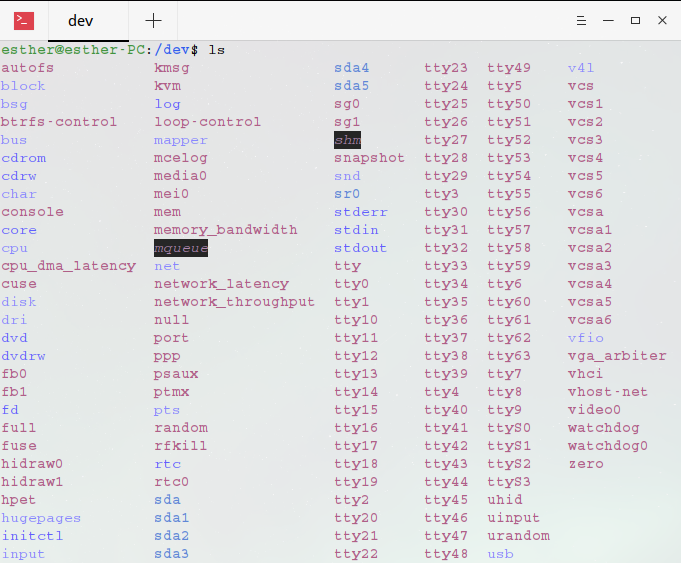
\includegraphics[scale = 0.4]{capitulo_03/figuras_dir/dev.jpg}
\caption{``hidraw0'' y ``hidraw1'' en {\itshape /dev}}
%\label{fig:figura4}
\end{figure}

Cada dispositivo USB HID tiene dos interfaces ``Hidraw'': ``Hidraw0'' y ``Hidraw1''. Cuando se realiza la llamada al sistema con {\itshape open()}, hay que conocer cúal de las dos corresponde al teclado y al ratón. Si la operación de apertura se realiza con éxito, se obtiene un descriptor de archivo que es un número entero pequeño, que normalmente es ``0'' para el teclado y ``3'' o superior para el ratón. El descriptor ``0'' es el que se le asigna a la  entrada estándar\footnote{La constante que representa la entrada estándar es ``stdin''. También se puede especificar la ruta del correspondiente archivo ``Hidraw''} y, de forma normal, los descriptores ``1'' y ``2'' se asocian a las salidas estándar\footnote{La constante que representa la salida estándar es ``stdout'' y la salida de error estándar es ``stderr''.} asignadas a la pantalla. El descriptor ``0'' pertenece a un archivo que se encuentra siempre abierto por el sistema considerado como la interfaz de entrada de eventos de dispositivos HID por defecto.

Como se ha comentado en la sección 2.8.1, Raspbian ofrece un manual que aporta información sobre las llamadas al sistema que se realizan con archivos. Cuando la aplicación tiene que manejar eventos de naturaleza distinta o, dicho de otro modo, que procedan de dos dispositivos distintos, interviene un proceso de demultiplexación. Por este proceso se entiende la evaluación de los descriptores de archivo que consiste en comprobar si estos cambian de estado. Este cambio se debe a movimientos de ratón y pulsaciones de tecla. La demultiplexación se lleva a cabo mediante una llamada al sistema con la función {\itshape select()}. A través de esta función, se determina qué descriptor va a ser leído cuando se detectan cambios en ambos descriptores.

En este caso, el programa comienza obteniendo los descriptores de los archivos ``Hidraw''. Tras esto, se definen dos variables de tipo ``fd\_set'' y se les hace coincidir sus direcciones de memoria. Posteriormente, se inicializa su contenido a cero con ``FD\_ZERO'' y se iguala al de los descriptores obtenidos con {\itshape open()} mediante ``FD\_SET'' a modo de inicialización. A continuación, se inicia un bucle infinito en el que, en cada iteracción, se realiza una lectura de uno de los dos descriptores. Este hecho está determinado por {\itshape select()}, cuya función toma como argumentos el descriptor más grande de los dos más una unidad\footnote{Este argumento especifica el rango de descriptores de archivo cuyo estado es comprobado por la función {\itshape select()}. El hecho de añadir un ``1'' se debe a que, de no ser así, esta función comprobaría el estado del descriptor 0 hasta el descriptor incluido en el argumento menos la unidad.}, el puntero a las variables definidas de tipo ``fd\_set'' y ``NULL'', en el resto. ``FD\_ISSET'' devuelve un valor distinto de cero si el valor del descriptor coincide con el valor asignado a la variable ``copia''. Cuando sucede esto, la variable entera ``fd'' toma el mismo valor que el descriptor se se procede a leer en las siguientes líneas de código. En caso contrario, devuelve un ``0''. 

Cuando se determina el dispositivo HID que se va a leer, se crea un vector de 1024 bytes de longitud. A continuación, se realiza una llamada al sistema con la función {\itshape read()} que se encarga de leer hasta 1024 bytes del archivo cuyo descriptor es ``fd'' introduciendo el contenido leído en el búfer creado. A su vez, esta función devuelve un número entero que corresponde al número de bytes leídos y mediante un bucle, se representa en hexadecimal cada byte leído (``Listing \ref{Lis: HidraweventosHID}'').


\begin{listing}[p]
\begin{minted}[bgcolor=bg,
               frame=lines,
               framesep=2mm,
               linenos
               ]
               {C}
    #include <sys/types.h>
    #include <sys/stat.h>
    #include <fcntl.h>
    #include <unistd.h>
    #include <stdio.h>
    #include <sys/select.h>
    
    int main() {
    	int teclado = open("/dev/hidraw0", O_RDONLY);
    	int raton = open("/dev/hidraw1", O_RDONLY);
    
    	fd_set *fds1;
    	fd_set fds2;
    	fds1=&fds2;
    	FD_ZERO(fds1);
    	FD_ZERO(&fds2);
    	FD_SET(teclado, fds1);
    	FD_SET(raton, &fds2);
    	
    	if (teclado<0 || raton<0)
    	printf("Error al abrir los archivos\n");
    	
    	for(;;) {
    		fd_set copia = fds2;
    		int n = select(raton+1, &copia, NULL, NULL, NULL);
    		int fd = -1;
    
    		if (FD_ISSET(teclado, &copia))
    			fd = teclado;
    
    		if (FD_ISSET(raton, &copia))
    			fd = raton;
    
    		char buf[1024];
    		n = read(fd, buf, 1024);
    
    		printf("%d ", n);
    		for(int i=0; i<n; ++i) {
    			printf("%x", buf[i]);
    		}
    		puts("");
    		if (n<0)
    			perror("Al leer");
    	}
    	return 0;
    }
\end{minted}
\caption{Programa de lectura y demultiplexación de eventos con ``Hidraw''}
\label{Lis: HidraweventosHID}
\end{listing}


Como resultado, la aplicación muestra los datos en hexadecimal de los movimientos del ratón y pulsaciones de teclas. Sin embargo, este programa no está sujeto a un patrón de programación, por lo que podría complicarse ni tampoco se pueden implementar excepciones de una manera sencilla. Es por esto por lo que se ha decidido que el proyecto se implemente con la biblioteca ``Reactor''.


%%%%%%%%%%%%%%%%%%%%% Subsección %%%%%%%%%%%%%%%%%%%%%
\subsection{Lectura y demultiplexado de eventos teclado - ratón con ``Reactor''} \label{s3_1_2}

%/////////////////// Subsubsección ///////////////////%
\subsubsection{Lectura de eventos de teclado}\label{s3_1_2_1}

``Reactor'' aporta una forma sencilla de obtener los eventos de estos periféricos. Con este ejemplo, obtenido del libro del taller \citep[pág. 98--99]{tallerRPi}, se recogen los eventos producidos por el teclado:

\begin{listing}[H]
\begin{minted}[bgcolor=bg,
               frame=lines,
               framesep=2mm,
               linenos]
               {C}
    #include <reactor/reactor.h>
    #include <reactor/console.h>
    #include <stdio.h>
    #include <unistd.h>
    
    static void keyboard (event_handler* ev);
   
    event_handler* keyboard_handler_new() {
    	return event_handler_new(0, keyboard);
    }
    
    static void keyboard (event_handler* ev) {
    	char buf[1];
    	if (read (ev->fd, buf, 1) <0 || buf[0]=='q')
    		reactor_quit(ev->r);
    	printf("pulsando %c\n", buf[0]);
    }
    
    int main () {
    	
    	void* state= console_set_raw_mode(0);
    	reactor *r= reactor_new();
    	reactor_add(r, keyboard_handler_new());
    	reactor_run(r);
    	console_restore(0,  state);
    	return 0;
    	
    }

\end{minted}
\caption{Programa de lectura de eventos de teclado con ``Reactor''}
\label{Lis: eventostecladoreactor}
\end{listing}
\clearpage

En primer lugar, se llama a la función ``console\_set\_raw\_mode()'' que permite que al pulsar teclas en el terminal, automáticamente sean procesadas como eventos sin tener que pulsar sobre ``enter'', esperar un tiempo o sobrepasar un número máximo de caracteres. Seguidamente, se crea un puntero a un objeto de tipo ``reactor'' y se inicializan los atributos mediante ``reactor\_new()''. Posteriormente, mediante ``reactor\_add()'' se introduce el manejador en el objeto de tipo ``reactor'' apuntado por ``r'' y se inicia el bucle de eventos con ``reactor\_run()'', con el cual se accede a la llamada al sistema {\itshape select()} para multiplexar eventos eligiendo aquellos que se van a enviar al correspondiente manejador. En este caso, existe un solo manejador para despachar los eventos del teclado: ``keyboard\_handler\_new()''. \\
``keyboard\_handler\_new()'' es una función que devuelve un puntero de tipo ``event\_handler'' a un objeto creado por ``event\_handler\_new()'' en el cual, figuran como argumentos el descriptor del archivo ``Hidraw'' correspondiente y una función que se ejecuta cada vez que se invoca al manejador. Esta función llamada ``keyboard'' accede al archivo descriptor que apunta el objeto manejador y mediante {\itshape read()} lee el contenido para mostrar los eventos por pantalla. Si esta función devuelve un ``1'' o se pulsa a la tecla ``q'', entonces el bucle de eventos se detiene. Finalmente, ``console\_restore()'' reestablece la configuración anterior que fue modificada por ``console\_set\_raw\_mode()''. 



%/////////////////// Subsubsección ///////////////////%
\subsubsection{Lectura de eventos de ratón}\label{s3_1_2_2}

Este programa es similar al anterior. Lo único que hay que tener en cuenta es que el descriptor del ratón no es el mismo que el de la entrada estándar, por tanto es necesario obtenerlo e introducirlo en ``event\_handler\_new()'' para que cree el manejador y registre el descriptor en el objeto que posteriormente se usa para la lectura (``Listing \ref{Lis: eventosratonreactor}''). 

\begin{listing}[p]
\begin{minted}[bgcolor=bg,
               frame=lines,
               framesep=2mm,
               linenos]
               {C}
    #include <reactor/reactor.h>
    #include <reactor/console.h>
    #include <stdio.h>
    #include <unistd.h>
    #include <assert.h>
    #include <sys/types.h>
    #include <sys/stat.h>
    #include <fcntl.h>
    #include <sys/select.h>
    
    
    static void mouse (event_handler* ev);
    
    event_handler* mouse_handler_new(int fd) {
    	return event_handler_new(fd, mouse);
    }
    
    static void mouse (event_handler* ev) {
    	printf("ev->fd %d\n",ev->fd);
    	char buf[1024];
    	int p= read (ev->fd, buf, 1024);
    	printf("bytes: %d\n", p);
    	if (p <0)
    		reactor_quit(ev->r);
    		
    	for(int i=0; i<p; ++i) {
    		printf("%x", buf[i]);
    	}
    	puts("");
    }
    
    int main () {
    	
    	int fd1 = open("/dev/hidraw1", O_RDONLY);
    	
    	void* state= console_set_raw_mode(0);
    	reactor *r= reactor_new();
    	reactor_add(r, mouse_handler_new(fd1));
    	reactor_run(r);
    	console_restore(0,  state);
    	return 0;
    	
    }

\end{minted}
\caption{Programa de lectura de eventos de ratón con ``Reactor''}
\label{Lis: eventosratonreactor}
\end{listing}



%/////////////////// Subsubsección ///////////////////%
\subsubsection{Demultiplexado de eventos}\label{s3_1_2_3}

Una vez que ya se sabe cómo obtener los eventos de ambos dispositivos, se puede desarrollar un programa que tome todos los eventos y los demultiplexe enviándolos a los manejadores oportunos que se encargan de leerlos y mostrarlos por pantalla. Para ello, solamente se necesita un puntero a un objeto de tipo ``Reactor''. Este objeto registra ambos eventos con ``reactor\_add()'' y después, comienza la demultiplexación una vez iniciado el bucle de eventos (``Listing \ref{Lis: eventosdemultiplexados}''). 

Tras demultiplexar los eventos, el manejador correspondiente se encarga de mostrar los eventos por pantalla en el terminal y de abrir un archivo especial para escribir los bytes que conforman los eventos. Este conjunto de bytes se escriben precedidos de un carácter: ``T'' en caso de ser un evento del teclado y ``R'' en caso de ser un evento de ratón. La finalidad de esto consiste en que el programa que lea el contenido del archivo FIFO (``Cliente.c'') sepa identificar el tipo de evento que se ha escrito en él.


\begin{listing}
\begin{minted}[bgcolor=bg,
               frame=lines,
               framesep=2mm,
               linenos]
               {C}
    #include <reactor/reactor.h>
    #include <reactor/console.h>
    #include <stdio.h>
    #include <unistd.h>
    #include <assert.h>
    #include <sys/types.h>
    #include <sys/stat.h>
    #include <fcntl.h>
    #include <sys/select.h>
    
    static void keyboard (event_handler* ev);
    static void mouse (event_handler* ev);
    event_handler* mouse_handler_new(int fd) {
    	return event_handler_new(fd, mouse);
    }
    static void mouse (event_handler* ev) {
    	int fifo= -1;	
    	fifo = open("archivo", O_RDWR|O_NONBLOCK);
    	unsigned char bufer[1024];
    	int p= read (ev->fd, bufer, 1024);
    	int a, t= 0;      
    	if (p <0)
    		reactor_quit(ev->r);
    	typedef struct raton{
    	char tipo;
    	unsigned char buf[1024];
    	} movimiento;
    	movimiento evento;
    	evento.tipo = 'R';
  
    	for(int i=0; i<p; ++i) {
    	evento.buf[i] = bufer[i];
    	}
    	for(t=0; t<p; ++t) {
    		printf("%x", evento.buf[t]);
    		printf(" - ");
    	}
    	puts("");
    	a= write(fifo, &evento, p+1);
    	close(fifo);
    }
\end{minted}
\caption{Continuación de ``Listing \ref{Lis: eventosdemultiplexados}''}
%\label{Lis: eventosdemultiplexados}
\end{listing}
    
    
\begin{listing}[p]
\begin{minted}[bgcolor=bg,
               frame=lines,
               framesep=2mm,
               linenos]
               {C} 
    event_handler* keyboard_handler_new() {
    	return event_handler_new(0, keyboard);
    }
    static void keyboard (event_handler* ev) {
	int fifo= -1;	
	fifo = open("archivo", O_RDWR|O_NONBLOCK);
	char bufer[1];
	int s= read (ev->fd, bufer, sizeof(bufer));
	if (s <0 || bufer[0]=='q')
		reactor_quit(ev->r);
	printf("pulsando %c\n", bufer[0]);

	typedef struct teclado{
	char tipo;
	char buf[1];
	} tecla;
	tecla pulsacion;
	pulsacion.tipo = 'T';
	pulsacion.buf[0]=bufer[0];
	int d;
	d= write(fifo, &pulsacion, sizeof(pulsacion));
	close(fifo);
    }
    
    int main () {
    	
    	int fd1 = open("/dev/hidraw1", O_RDONLY);
    	void* state= console_set_raw_mode(0);
    	reactor *r= reactor_new();
    	reactor_add(r, keyboard_handler_new());
    	reactor_add(r, mouse_handler_new(fd1));
    	reactor_run(r);
    	console_restore(0,  state);
    	return 0;
    }
\end{minted}
\caption{Programa de lectura y demultiplexado de eventos con ``Reactor''}
\label{Lis: eventosdemultiplexados}
\end{listing}

\clearpage
%\newpage
%%%%%%%%%%%%%%%%%%%%%%%%%%%%%%%%%%%%%%%%%%%%%%%%%%%%%%%
%		            	Seccion          			  %
%%%%%%%%%%%%%%%%%%%%%%%%%%%%%%%%%%%%%%%%%%%%%%%%%%%%%%%
\section{Seguimiento ocular} \label{s3_2}

%%%%%%%%%%%%%%%%%%%%% Subsección %%%%%%%%%%%%%%%%%%%%%
\subsection{Captura de eventos faciales y oculares con ``eye\_detect.cpp''} \label{s3_2_1}

Para que el sistema conozca el lugar hacia donde mira el usuario, se requiere algún tipo de aplicación capaz de detectar la posición de los ojos. Existen numerosas aplicaciones desarrolladas por la comunidad de desarrolladores de software libre con OpenCV, entre ellos, cabe destacar el sistema de seguimiento ocular o ``eye tracking'' implementado en C++ por Abner Matheus el cual está expuesto y perfectamente explicado en su blog \citep{eyetracking}.

El programa se divide en las siguientes partes\footnote{El análisis se realiza en el mismo orden en que está elaborado el programa.}:

\begin{itemize}

    \item Carga de librerías: 

\begin{listing}[h]
\begin{minted}[bgcolor=bg,
               frame=lines,
               framesep=2mm,
               linenos]
               {C}
    #include <iostream>

    #include <opencv2/core/core.hpp>
    #include <opencv2/highgui/highgui.hpp>
    #include <opencv2/imgproc/imgproc.hpp>
    #include <opencv2/objdetect/objdetect.hpp>
    
    #include <sys/types.h>
    #include <sys/stat.h>
    #include <fcntl.h>
    #include <unistd.h>


\end{minted}
\caption{Archivos cabecera de ``eye\_detect.cpp''}
\label{Lis: libreriasopencv}
\end{listing}


    
    Se cargan los archivos cabecera de:
    \begin{itemize}
        \item La biblioteca del sistema (types.h, stat.h, fcntl.h y unistd.h) para poder abrir y escribir en un archivo FIFO.
        \item La biblioteca estándar STL (iostream) para operaciones de entrada y salida.
        \item Las bibliotecas de OpenCV (core.hpp, highgui.hpp, imgproc.hpp y objdetect.hpp).
    \end{itemize}
    
\clearpage
   \item Detección del iris:

\begin{listing}[H]
\begin{minted}[bgcolor=bg,
               frame=lines,
               framesep=2mm,
               linenos]
               {C}
int fifo = -1;

    cv::Vec3f getEyeball(cv::Mat &eye, std::vector<cv::Vec3f> &circles)
    {
      std::vector<int> sums(circles.size(), 0);
      for (int y = 0; y < eye.rows; y++)
      {
          uchar *ptr = eye.ptr<uchar>(y);
          for (int x = 0; x < eye.cols; x++)
          {
              int value = static_cast<int>(*ptr);
              for (int i = 0; i < circles.size(); i++)
              {
                  cv::Point center((int)std::round(circles[i][0]), (int)std::round(circles[i][1]));
                  int radius = (int)std::round(circles[i][2]);
                  if (std::pow(x - center.x, 2) + std::pow(y - center.y, 2) < std::pow(radius, 2))
                  {
                      sums[i] += value;
                  }
              }
              ++ptr;
          }
      }
      int smallestSum = 9999999;
      int smallestSumIndex = -1;
      for (int i = 0; i < circles.size(); i++)
      {
          if (sums[i] < smallestSum)
          {
              smallestSum = sums[i];
              smallestSumIndex = i;
          }
      }
      return circles[smallestSumIndex];
    }
\end{minted}
\caption{Detección del iris}
\label{Lis: deteccioniris}
\end{listing}
    En primer lugar, se crea el descriptor de un archivo FIFO y lo inicializa a ``-1''. Seguidamente, la función ``getEyeball()'' selecciona la región circular que contiene más cantidad de píxeles negros (pupila).
    
    \item Selección del ojo izquierdo: 
    
\begin{listing}[H]
\begin{minted}[bgcolor=bg,
               frame=lines,
               framesep=2mm,
               linenos]
               {C}
    cv::Rect getLeftmostEye(std::vector<cv::Rect> &eyes)
    {
      int leftmost = 99999999;
      int leftmostIndex = -1;
      for (int i = 0; i < eyes.size(); i++)
      {
          if (eyes[i].tl().x < leftmost)
          {
              leftmost = eyes[i].tl().x;
              leftmostIndex = i;
          }
      }
      return eyes[leftmostIndex];
    }
\end{minted}
\caption{Selección del ojo izquierdo}
\label{Lis: deteccionojoizq}
\end{listing}
    
La función ``getLeftmostEye()'' devuelve un objeto de la clase ``cv::Rect'' que proporciona las coordenadas de la esquina superior izquierda del área rectangular que encierra el ojo junto a la altura y a la anchura del mismo (``Listing \ref{Lis: deteccionojoizq}'').

    \item Estabilización de las coordenadas del iris: 
    
\begin{listing}[H]
\begin{minted}[bgcolor=bg,
               frame=lines,
               framesep=2mm,
               linenos]
               {C}
    std::vector<cv::Point> centers;
    
    cv::Point stabilize(std::vector<cv::Point> &points, int windowSize)
    {
      float sumX = 0;
      float sumY = 0;
      int count = 0;
\end{minted}
\caption{Continuación de Listing \ref{Lis: estabilizacion}}
%\label{Lis: estabilizacion}
\end{listing}

\begin{listing}[H]
\begin{minted}[bgcolor=bg,
               frame=lines,
               framesep=2mm,
               linenos]
               {C}
      for (int i = std::max(0, (int)(points.size() - windowSize)); i < points.size(); i++)
      {
          sumX += points[i].x;
          sumY += points[i].y;
          ++count;
      }
      if (count > 0)
      {
          sumX /= count;
          sumY /= count;
      }
      return cv::Point(sumX, sumY);
    }
    
\end{minted}
\caption{Estabilización de las coordenadas del iris}
\label{Lis: estabilizacion}
\end{listing}

Esta función realiza la media de las coordenadas del iris que se obtienen en las últimas cinco detecciones para obtener las coordenadas más precisas, ya que el algoritmo encargado de la detección de regiones circulares dentro del área cuadrada del ojo es bastante inestable (``Listing \ref{Lis: estabilizacion}'').

    \item Detección del área rectangular que contiene los ojos: 

Esta función es la más importante de todo el programa (``Listing \ref{Lis: arearectangular}''). Recibe como argumentos las imágenes detectadas por la cámara en una matriz denominada ``frame'' y los dos clasificadores de clase ``cv::CascadeClassifier''. En primer lugar, la imagen se convierte en otra imagen en escala de grises mediante ``cv::cvtColor''. Posteriormente, se mejora el contraste de la imagen para que las clasificaciones sean más precisas. A continuación, se crea un vector de objetos de la clase ``Rect'' para almacenar las coordenadas de la esquina superior del recuadro que contiene la cara denominado ``faces''. El proceso de detección del rostro se lleva a cabo mediante ``faceCascade.detectMultiScale()'' en el cual, el vector ``faces'' se rellena con la información obtenida en la clasificación y después, una claúsula `ìf'' evalúa si este vector está vacío o no. Si se da el primer caso, significa que no ha sido posible detectar el rostro.

Cuando se ha detectado la cara, se define una matriz con la clase ``cv::Mat'' llamada ``face'' que contiene la información relativa a la región de la cara, ignorando aquella en la cual la clasificación haya dado como resultado zonas sin cara o negativas. Sobre este área se realiza de nuevo una clasificación con los clasificadores de detección de ojos. Para ello, se define el vector ``eyes'' y la clasificación comienza cuando se llama a ``eyeCascade.detectMultiScale()''.

\begin{listing}[p]
\begin{minted}[bgcolor=bg,
               frame=lines,
               framesep=2mm,
               linenos]
               {C}
    void detectEyes(cv::Mat &frame, cv::CascadeClassifier &faceCascade, cv::CascadeClassifier &eyeCascade)
    {
      cv::Mat grayscale;
      cv::cvtColor(frame, grayscale, CV_BGR2GRAY);
      cv::equalizeHist(grayscale, grayscale);
      std::vector<cv::Rect> faces;
      faceCascade.detectMultiScale(grayscale, faces, 1.1, 2, 0 | CV_HAAR_SCALE_IMAGE, cv::Size(150, 150));
      if (faces.size() == 0) return; 
      cv::Mat face = grayscale(faces[0]); 
      std::vector<cv::Rect> eyes;
      eyeCascade.detectMultiScale(face, eyes, 1.1, 2, 0 | CV_HAAR_SCALE_IMAGE, cv::Size(30, 30));   
      std::cout << "Face " << faces[0] << std::endl;
      rectangle(frame, faces[0].tl(), faces[0].br(), cv::Scalar(255, 0, 0), 2);
      if (eyes.size() != 2) return;
      for (cv::Rect &eye : eyes)
      {	
          rectangle(frame, faces[0].tl() + eye.tl(), faces[0].tl() + eye.br(), cv::Scalar(0, 255, 0), 2);
          std::cout << "Ojos" << eye << std::endl;
          struct {
            char type;
            cv::Rect eye;
          } s = {
            'E', eye
          };
          ::write(fifo, &s, sizeof(s));
      }
      cv::Rect eyeRect = getLeftmostEye(eyes);
      cv::Mat eye = face(eyeRect);
      cv::equalizeHist(eye, eye);
      std::vector<cv::Vec3f> circles;
      cv::HoughCircles(eye, circles, CV_HOUGH_GRADIENT, 1, eye.cols / 8, 250, 15, eye.rows / 8, eye.rows / 3);
\end{minted}
\caption{Continuación de ``Listing \ref{Lis: arearectangular}'')}
%\label{Lis: arearectangular}
\end{listing}
      
\begin{listing}[p]
\begin{minted}[bgcolor=bg,
               frame=lines,
               framesep=2mm,
               linenos]
               {C} 
      if (circles.size() > 0)
      {
          cv::Vec3f eyeball = getEyeball(eye, circles);
          cv::Point center(eyeball[0], eyeball[1]);
          centers.push_back(center);
          center = stabilize(centers, 5);
          int radius = (int)eyeball[2];
          std::cout << "Pupila " << center << ", " << radius << std::endl;
          
          
           struct {
            char type;
            cv::Point center;
            int radius;
           
          } p = {
            'P', center, radius
          };
          ::write(fifo, &p, sizeof(p));
          
          cv::circle(frame, faces[0].tl() + eyeRect.tl() + center, radius, cv::Scalar(0, 0, 255), 2);
          cv::circle(eye, center, radius, cv::Scalar(255, 255, 255), 2);
      }
      cv::imshow("Eye", eye);
    }

\end{minted}
\caption{Detección del área rectangular que contiene los ojos}
\label{Lis: arearectangular}
\end{listing}

A continuación, se muestran por pantalla los eventos obtenidos como coordenadas en el eje X e Y respecto al punto superior izquierdo del recuadro de la cara cuyas coordenadas están determinadas en base al origen situado en la esquina superior izquierda de la captura de vídeo desde el punto de vista de un observador situado en frente del monitor y se representa el rectángulo que engloba el área del rostro.

Después de esto, se realiza una comprobación para saber si ambos ojos se han detectado. Esto sucede cuando el tamaño del vector ``eyes'' es igual a ``2''. Si se da el caso en el que los dos ojos son detectados, comienza un bucle que se usa para dibujar los rectángulos de ambos ojos y para introducir tras cada proceso de detección los eventos o coordenadas de los mismos en un archivo especial FIFO y así poder usarlos en otros procesos (tubería). Para realizar esto, se crea un objeto cuyos atributos son el tipo de evento expresado por un carácter y un objeto de clase ``Rect'' que contiene los propios eventos. Éstos se introducen precedidos de un carácter en el archivo FIFO ``eye\_fifo'' a través de una llamada a {\itshape write()}. Este carácter indica el tipo de evento (cara, ojos o pupila) y sirve para identificar los datos relacionados con los ojos y así diferenciarlos de los de la cara o el iris.
    
El proceso que se sigue en la detección del iris es parecido al de los ojos: Se llama a la función ``getLeftmostEye()'' para obtener los eventos estabilizados del ojo izquierdo, se toma la región de la cara que contiene únicamente los ojos (``eye'') y en base a ella, se llama a ``HoughCircles()'', una función basada en un algoritmo que detecta las regiones circulares dentro de este área. Cuando detecta una zona circular, los datos correspondientes a esta zona se introducen en el vector ``circles''. El siguiente paso consiste en evaluar si este vector está vacío o no. En caso de no estarlo es porque el algoritmo anterior sí ha detectado una zona circular. Seguidamente, se invoca a ``getEyeball()'' que analiza la región circular y determina las coordenadas de la zona en la que hay mayor densidad de píxeles negros, cuya zona es considerada como la pupila. A su vez, este es el centro del iris, definido por el vector ``center''. La función termina con la impresión por pantalla y el envío al archivo FIFO de las coordenadas de la pupila y el radio junto con la representación de la región del iris.

    \item Función principal. Carga de clasificadores: 
    
    Se definen los clasificadores ``faceCascade'' y ``eyeCascade'' y se cargan con la extensión ``.load'' (``Listing \ref{Lis: cargaclasificadores}''). Estos clasificadores se encuentran en archivos independientes en formato ``.xml''. En el caso en que no se puedan cargar, se informa por pantalla del error y se devuelve el valor ``-1''.
    
\begin{listing}[p]
\begin{minted}[bgcolor=bg,
               frame=lines,
               framesep=2mm,
               linenos]
               {C} 
    int main(int argc, char **argv)
    {
      cv::CascadeClassifier faceCascade;
      cv::CascadeClassifier eyeCascade;
      if (!faceCascade.load("./haarcascade_frontalface_alt.xml"))
      {
          std::cerr << "Could not load face detector." << std::endl;
          return -1;
      }    
      if (!eyeCascade.load("./haarcascade_eye_tree_eyeglasses.xml"))
      {
          std::cerr << "Could not load eye detector." << std::endl;
          return -1;
      }
    
\end{minted}
\caption{Carga de clasificadores}
\label{Lis: cargaclasificadores}
\end{listing}

    \item Función principal. Encendido de la cámara:
    
\begin{listing}[p]
\begin{minted}[bgcolor=bg,
               frame=lines,
               framesep=2mm,
               linenos]
               {C} 

    cv::VideoCapture cap(0); 
    if (!cap.isOpened())
      {
          std::cerr << "Webcam not detected." << std::endl;
          return -1;
      }  
    
\end{minted}
\caption{Encendido de la cámara en ``eye\_detect.cpp''}
\label{Lis: camaraon}
\end{listing}
    
    En primer lugar, se define ``cap'' con la clase ``cv::VideoCapture'' del módulo ``highgui'' de OpenCV. Posteriormente, se enciende con la extensión ``.is0pened()''. En el caso de que la cámara no se haya detectado, se informa de la situación por pantalla y devuelve ``-1'' (``Listing \ref{Lis: camaraon}'').
    
\clearpage
    \item Función principal. Visualización de vídeo:

La imagen capturada por la cámara se convierte en una matriz. Si el contenido de esa matriz es nulo, el programa sale del bucle, en caso contrario, se hace una llamada a ``detectEyes()'' para obtener los eventos del ojo y la pupila e introducirlo en el archivo especial. Además, por cada iteración se hacen 30 capturas que se clasifican con los correspondientes clasificadores mediante el algoritmo de Viola-Jones.     

\begin{listing}[H]
\begin{minted}[bgcolor=bg,
               frame=lines,
               framesep=2mm,
               linenos]
               {C} 
    fifo = open("eye_fifo", O_WRONLY|O_CREAT, ~0);
    cv::Mat frame;
    while (1)
      {
          cap >> frame;
          if (!frame.data) break;
          detectEyes(frame, faceCascade, eyeCascade);
          cv::imshow("Webcam", frame);
          if (cv::waitKey(30) >= 0) break;
      }
      return 0;
    } 
    
\end{minted}
\caption{Visualización de vídeo en ``eye\_detect.cpp''}
\label{Lis: visualizacionvideo}
\end{listing}

    
\end{itemize}
 \clearpage
%%%%%%%%%%%%%%%%%%%%% Subsección %%%%%%%%%%%%%%%%%%%%%
\subsection{Calibración de la cámara} \label{s3_2_2}

%/////////////////// Subsubsección ///////////////////%
\subsubsection{Captura de imágenes con ``save\_capture.cpp''}\label{s3_2_2_1}

El primer paso en el proceso de calibración consiste en realizar varias capturas situando la plantilla en diferentes posiciones. De esta forma, al disponer de un gran número de muestras distintas, durante el proceso de calibración se analizan los puntos de los cuadrados en distintas orientaciones, lo cual otorga mayor precisión a la calibración.
La toma de las muestras o capturas se lleva a cabo con ``save\_capture.cpp’’. Las distintas partes del programa se describen a continuación:


\begin{itemize}
    \item Carga de librerías:
    
\begin{listing}[H]
\begin{minted}[bgcolor=bg,
               frame=lines,
               framesep=2mm,
               linenos]
               {C} 
    #include "opencv2/core.hpp"
    #include <opencv2/core/utility.hpp>
    #include "opencv2/imgproc.hpp"
    #include "opencv2/calib3d.hpp"
    #include "opencv2/imgcodecs.hpp"
    #include "opencv2/videoio.hpp"
    #include "opencv2/highgui.hpp"
    
    #include <stdio.h>
    #include <stdlib.h>
    #include <iostream>
    #include <string> 
    #include <sstream> 
\end{minted}
\caption{Carga de librerías en ``save\_capture.cpp''}
\label{Lis: visualizacionvideocal}
\end{listing}
    
    
En primer lugar, se cargan los módulos de OpenCV y posteriormente, algunos archivos cabecera de librerías comunes.

    \item Función principal. Encendido de la cámara:
    
\begin{listing}[p]
\begin{minted}[bgcolor=bg,
               frame=lines,
               framesep=2mm,
               linenos]
               {C} 
    using namespace cv;
    
    int main (){

    std::vector<int> compression_params;
    compression_params.push_back(CV_IMWRITE_JPEG_QUALITY);
    compression_params.push_back(100);
    
    Mat img;
    
    VideoCapture cam = VideoCapture(0);
    if(!cam.isOpened()){
    	printf("!No se pudo abrir la camara!\n");
    	getchar();//espera que se preione Enter para dejar seguir
    	return -1;
    	} 
\end{minted}
\caption{Encendido de la cámara en ``save\_capture.cpp''}
\label{Lis: camaraonsave}
\end{listing}
    
Se inicia la cámara y se comprueba si se detecta o no, de la misma forma que en ``eye\_detect.cpp’’ (``Listing \ref{Lis: camaraonsave}). 

    \item Función principal. Registro de la dirección: 
    
\begin{listing}[p]
\begin{minted}[bgcolor=bg,
               frame=lines,
               framesep=2mm,
               linenos]
               {C} 
    bool SaveImage;
	int nimgs = 0;
	std::string direccion = "//home//esther//Desktop//VKMS//Calibracion";
	std::stringstream Saveimgs;
\end{minted}
\caption{Registro de la dirección}
\label{Lis: direccion}
\end{listing}
    
Se declara e inicializa una cadena de caracteres que contiene la ruta en la que se almacenan las imágenes capturadas (``Listing \ref{Lis: direccion}'').
\clearpage
    \item Función principal. Bucle de capturas: 

\begin{listing}[H]
\begin{minted}[bgcolor=bg,
               frame=lines,
               framesep=2mm,
               linenos]
               {C} 
    for(;;){
    	
    cam >> img;
    	
    namedWindow("image",WINDOW_AUTOSIZE);
    imshow("image", img);
    	
    if(waitKey(30) == 13){//espera 30ms y pregunta por ENTER
    
    	Saveimgs << direccion << nimgs << ".jpg";
    	SaveImage = imwrite(Saveimgs.str().c_str(), img, compression_params);
    	Saveimgs = std::stringstream();
    	nimgs++;
    		if (!SaveImage){
    			printf("!image %d saved failed!\n",nimgs);
    
    		}else{
    			printf("!image %d saved successful!\n",nimgs);
    		}
    		if (nimgs == 14){break;}
    		}
    	}
\end{minted}
\caption{Bucle de capturas}
\label{Lis: buclecapturas}
\end{listing}
    
La captura realizada se convierte en una matriz definida con el nombre ``ìmg’’, a continuación, se muestra en una ventana la imagen de vídeo y espera hasta que se presiona ``enter’’. En ese momento, se realiza una captura que se le asigna el mismo nombre que la carpeta final indicada en la ruta con formato ``.jpg’’. Por ejemplo, la ruta especificada para guardar las imágenes es {\itshape ``//home//esther//Desktop//VKMS//Calibracion''}, así pues, las capturas se nombran ``Calibracion’’ seguido de un número entero que constituye un contador en el programa, cuya variable es ``nimgs’’. Después, se realiza una llamada a ``imwrite()’’ que se engarga de guardar la imagen con el nombre especificado. Una vez hecho esto, el contador ``nimgs’’ se incrementa en una unidad. Esto sucede cada vez que se ejecuta una captura. El programa sale del bucle cuando el contador es igual a 14, lo que significa que se nombran imágenes como ```CalibracionN.jpg’’ siendo ``N’’ un número entre 0 y 13, por tanto, permite guardar 14 imágenes. En cada iteración, se realiza una comprobación para conocer si la imagen se ha guarda con éxito o no y lo notifica en el terminal. Cuando el bucle finaliza, se espera a que el usuario pulse alguna tecla y el programa termina (``Listing \ref{Lis: buclecapturas}'').
    
\end{itemize}


%/////////////////// Subsubsección ///////////////////%
\subsubsection{Calibración con ``calibration.cpp''}\label{s3_2_2_2}

Una vez se hayan capturado y guardado todas las imágenes, comienza el proceso de calibración con ``calibration.cpp’’:

\begin{itemize}
    \item Carga de librerías
    
\begin{listing}[H]
\begin{minted}[bgcolor=bg,
               frame=lines,
               framesep=2mm,
               linenos]
               {C}  
    #include "opencv2/core.hpp"
    #include <opencv2/core/utility.hpp>
    #include "opencv2/imgproc.hpp"
    #include "opencv2/calib3d.hpp"
    #include "opencv2/imgcodecs.hpp"
    #include "opencv2/videoio.hpp"
    #include "opencv2/highgui.hpp"
    
    #include <stdio.h>
    #include <stdlib.h>
    #include <iostream>
    #include <string> 
    #include <sstream>
\end{minted}
\caption{Carga de archivos cabecera en ``calibration.cpp’’}
\label{Lis: cabeceracali}
\end{listing}
    
    
    \item Cálculo de la posición de las esquinas de la plantilla (``Listing \ref{Lis: posicionesquinas}'')
    
\begin{listing}[p]
\begin{minted}[bgcolor=bg,
               frame=lines,
               framesep=2mm,
               linenos]
               {C}
    using namespace cv;

    static void calcChessboardCorners(Size boardSize, float squareSize, std::vector<cv::Point3f>& corners)
    {
    	corners.clear();
        for( int i = 0; i < boardSize.height; i++ )
            for( int j = 0; j < boardSize.width; j++ )
                corners.push_back(Point3f(float(j*squareSize),
                                          float(i*squareSize), 0)); 
    }
\end{minted}
\caption{Cálculo de la posición de las esquinas de la plantilla}
\label{Lis: posicionesquinas}
\end{listing}

    \item Guardado de los parámetros de la cámara (``Listing \ref{Lis: guardado}'')

\begin{listing}[p]
\begin{minted}[bgcolor=bg,
               frame=lines,
               framesep=2mm,
               linenos]
               {C}
    static void saveparams(const std::string& filename, 
        const Mat& cameraMatrix, const Mat& distCoeffs,
    	const std::vector<Mat>& rvecs,
    	const std::vector<Mat>& tvecs, 
    	const double& RMS)
    {
    FileStorage fs( filename, FileStorage::WRITE );
    fs << "Calibrate_Accuracy" << RMS;
    fs << "Camera_Matrix" << cameraMatrix;
    fs << "Distortion_Coefficients" << distCoeffs;
    fs << "Rotation_Vector" << rvecs;
    fs << "Translation_vector" << tvecs;
    
    if( !rvecs.empty() && !tvecs.empty() ){
    
    	CV_Assert(rvecs[0].type() == tvecs[0].type());
    	Mat bigmat((int)rvecs.size(), 6, rvecs[0].type());
    	for( int i = 0; i < (int)rvecs.size(); i++ ){
    		Mat r = bigmat(Range(i, i+1), Range(0,3));
    		Mat t = bigmat(Range(i, i+1), Range(3,6));
    
    		CV_Assert(rvecs[i].rows == 3 && rvecs[i].cols == 1);
    		CV_Assert(tvecs[i].rows == 3 && tvecs[i].cols == 1);
          
    			r = rvecs[i].t();
    			t = tvecs[i].t();
        }
        cvWriteComment( *fs, "Rotation vector + Translation vector", 0 );
        fs << "extrinsic_parameters" << bigmat;
        }
    		fs.release();
    }
\end{minted}
\caption{Guardado de los parámetros de la cámara}
\label{Lis: guardado}
\end{listing}
    
Determina el formato de guardado de la matriz de la cámara, los coeficientes de distorsión, el vector de rotación y el vector de traslación. Después concatena los vectores de traslación y rotación para formar la matriz de parámetros extrínsecos.
    
    \item Función principal. Definición de parámetros (``Listing \ref{Lis: definicion}'')
    
Se declaran los vectores que se van a usar como argumentos de las funciones a las que se llama y se define la variable ``patternsize’’ que toma el valor asignado por ``Size()’’ cuyos argumentos son el número de las esquinas interiores horizontales y verticales respectivamente. 
La plantilla que se ha usado es la que se muestra en la figura \ref{fig: plantilla}.
    
\begin{listing}[p]
\begin{minted}[bgcolor=bg,
               frame=lines,
               framesep=2mm,
               linenos]
               {C}
    int main(){
    
    cv::Size patternsize = cv::Size(9,6);
    std::vector<cv::Point3f> corners3D;
    std::vector<cv::Point2f> corners2D;
    std::vector<std::vector<cv::Point2f>> coord2D;
    std::vector<std::vector<cv::Point3f>> coord3D;
\end{minted}
\caption{Definición de parámetros}
\label{Lis: definicion}
\end{listing}
\clearpage


\begin{figure}
\centering
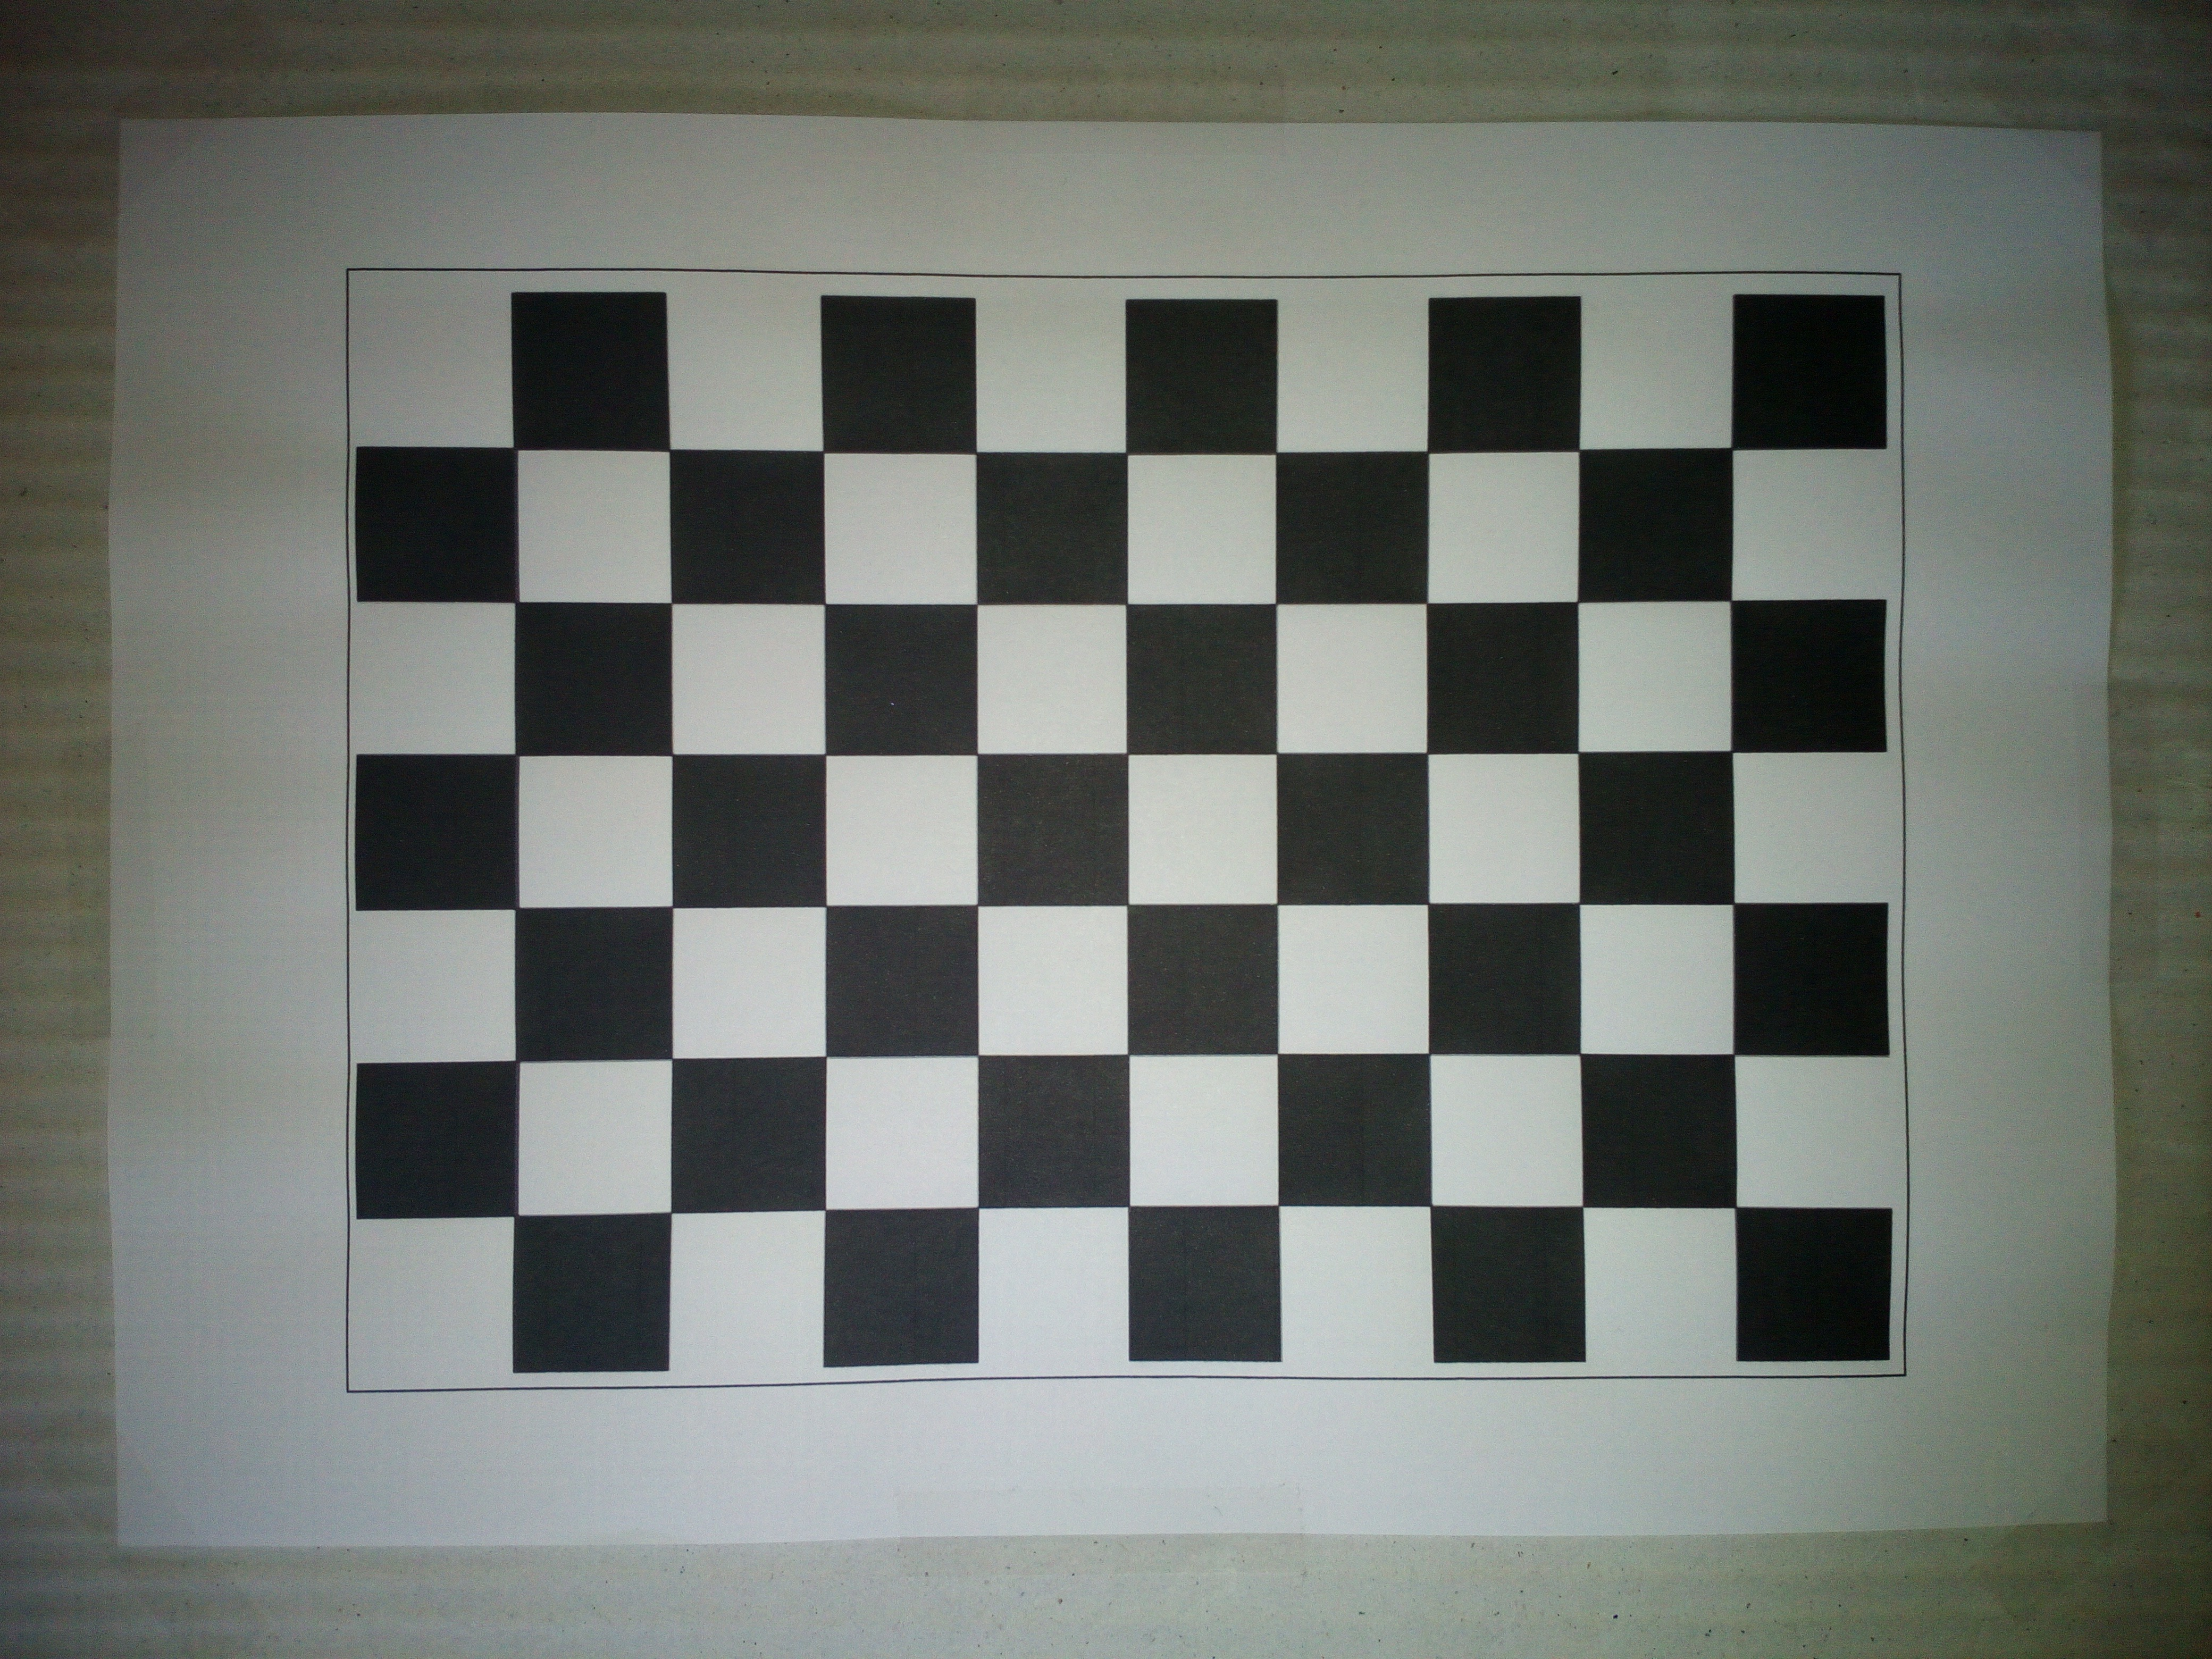
\includegraphics[scale = 0.05]{capitulo_03/figuras_dir/plantillazhang.jpg}
\caption{Plantilla Zhang usada en el proyecto}
\label{fig: plantilla}
\end{figure}
    
Como se puede observar, este patrón presenta ``9'' esquinas interiores horizontales y ``6'' esquinas interiores verticales.
    
    
    \item Función principal. Indicación de la ruta de las imágenes

\begin{listing}[H]
\begin{minted}[bgcolor=bg,
               frame=lines,
               framesep=2mm,
               linenos]
               {C}
    std::string direccion = "//home//esther//Desktop//VKMS//Calibracion//Calibracion";
    std::stringstream imgs;
\end{minted}
\caption{Ruta de las imágenes}
\label{Lis: indicacion}
\end{listing}
    
Se establece la ruta en la que se encuentran almacenadas las imágenes que se van a cargar después. El último conjunto de caracteres de la dirección corresponde con el nombre de las capturas sin contar con el número ``N’’ mencionado en el apartado anterior.

    \item Función principal. Llamada a la función ``calcChessbiardCorners()''
    
\begin{listing}[H]
\begin{minted}[bgcolor=bg,
               frame=lines,
               framesep=2mm,
               linenos]
               {C}
    calcChessboardCorners(patternsize,23,corners3D);
\end{minted}
\caption{Llamada a la función ``calcChessbiardCorners()''}
\label{Lis: calcChessbiardCorners}
\end{listing}

El segundo argumento debe modificarse en función de las características de la plantilla. Con ``características’’ se hace referencia a la longitud del lado de los cuadrados ya que este valor no es el mismo en todas ellas (varía en función de la escala con la que se imprima). Por tanto, este argumento constituye la longitud de los lados expresada en milímetros. En este caso, cada cuadrado mide 23 milímetros (figura \ref{fig: dimensioncuadrados}).

    \begin{figure}
    \centering
    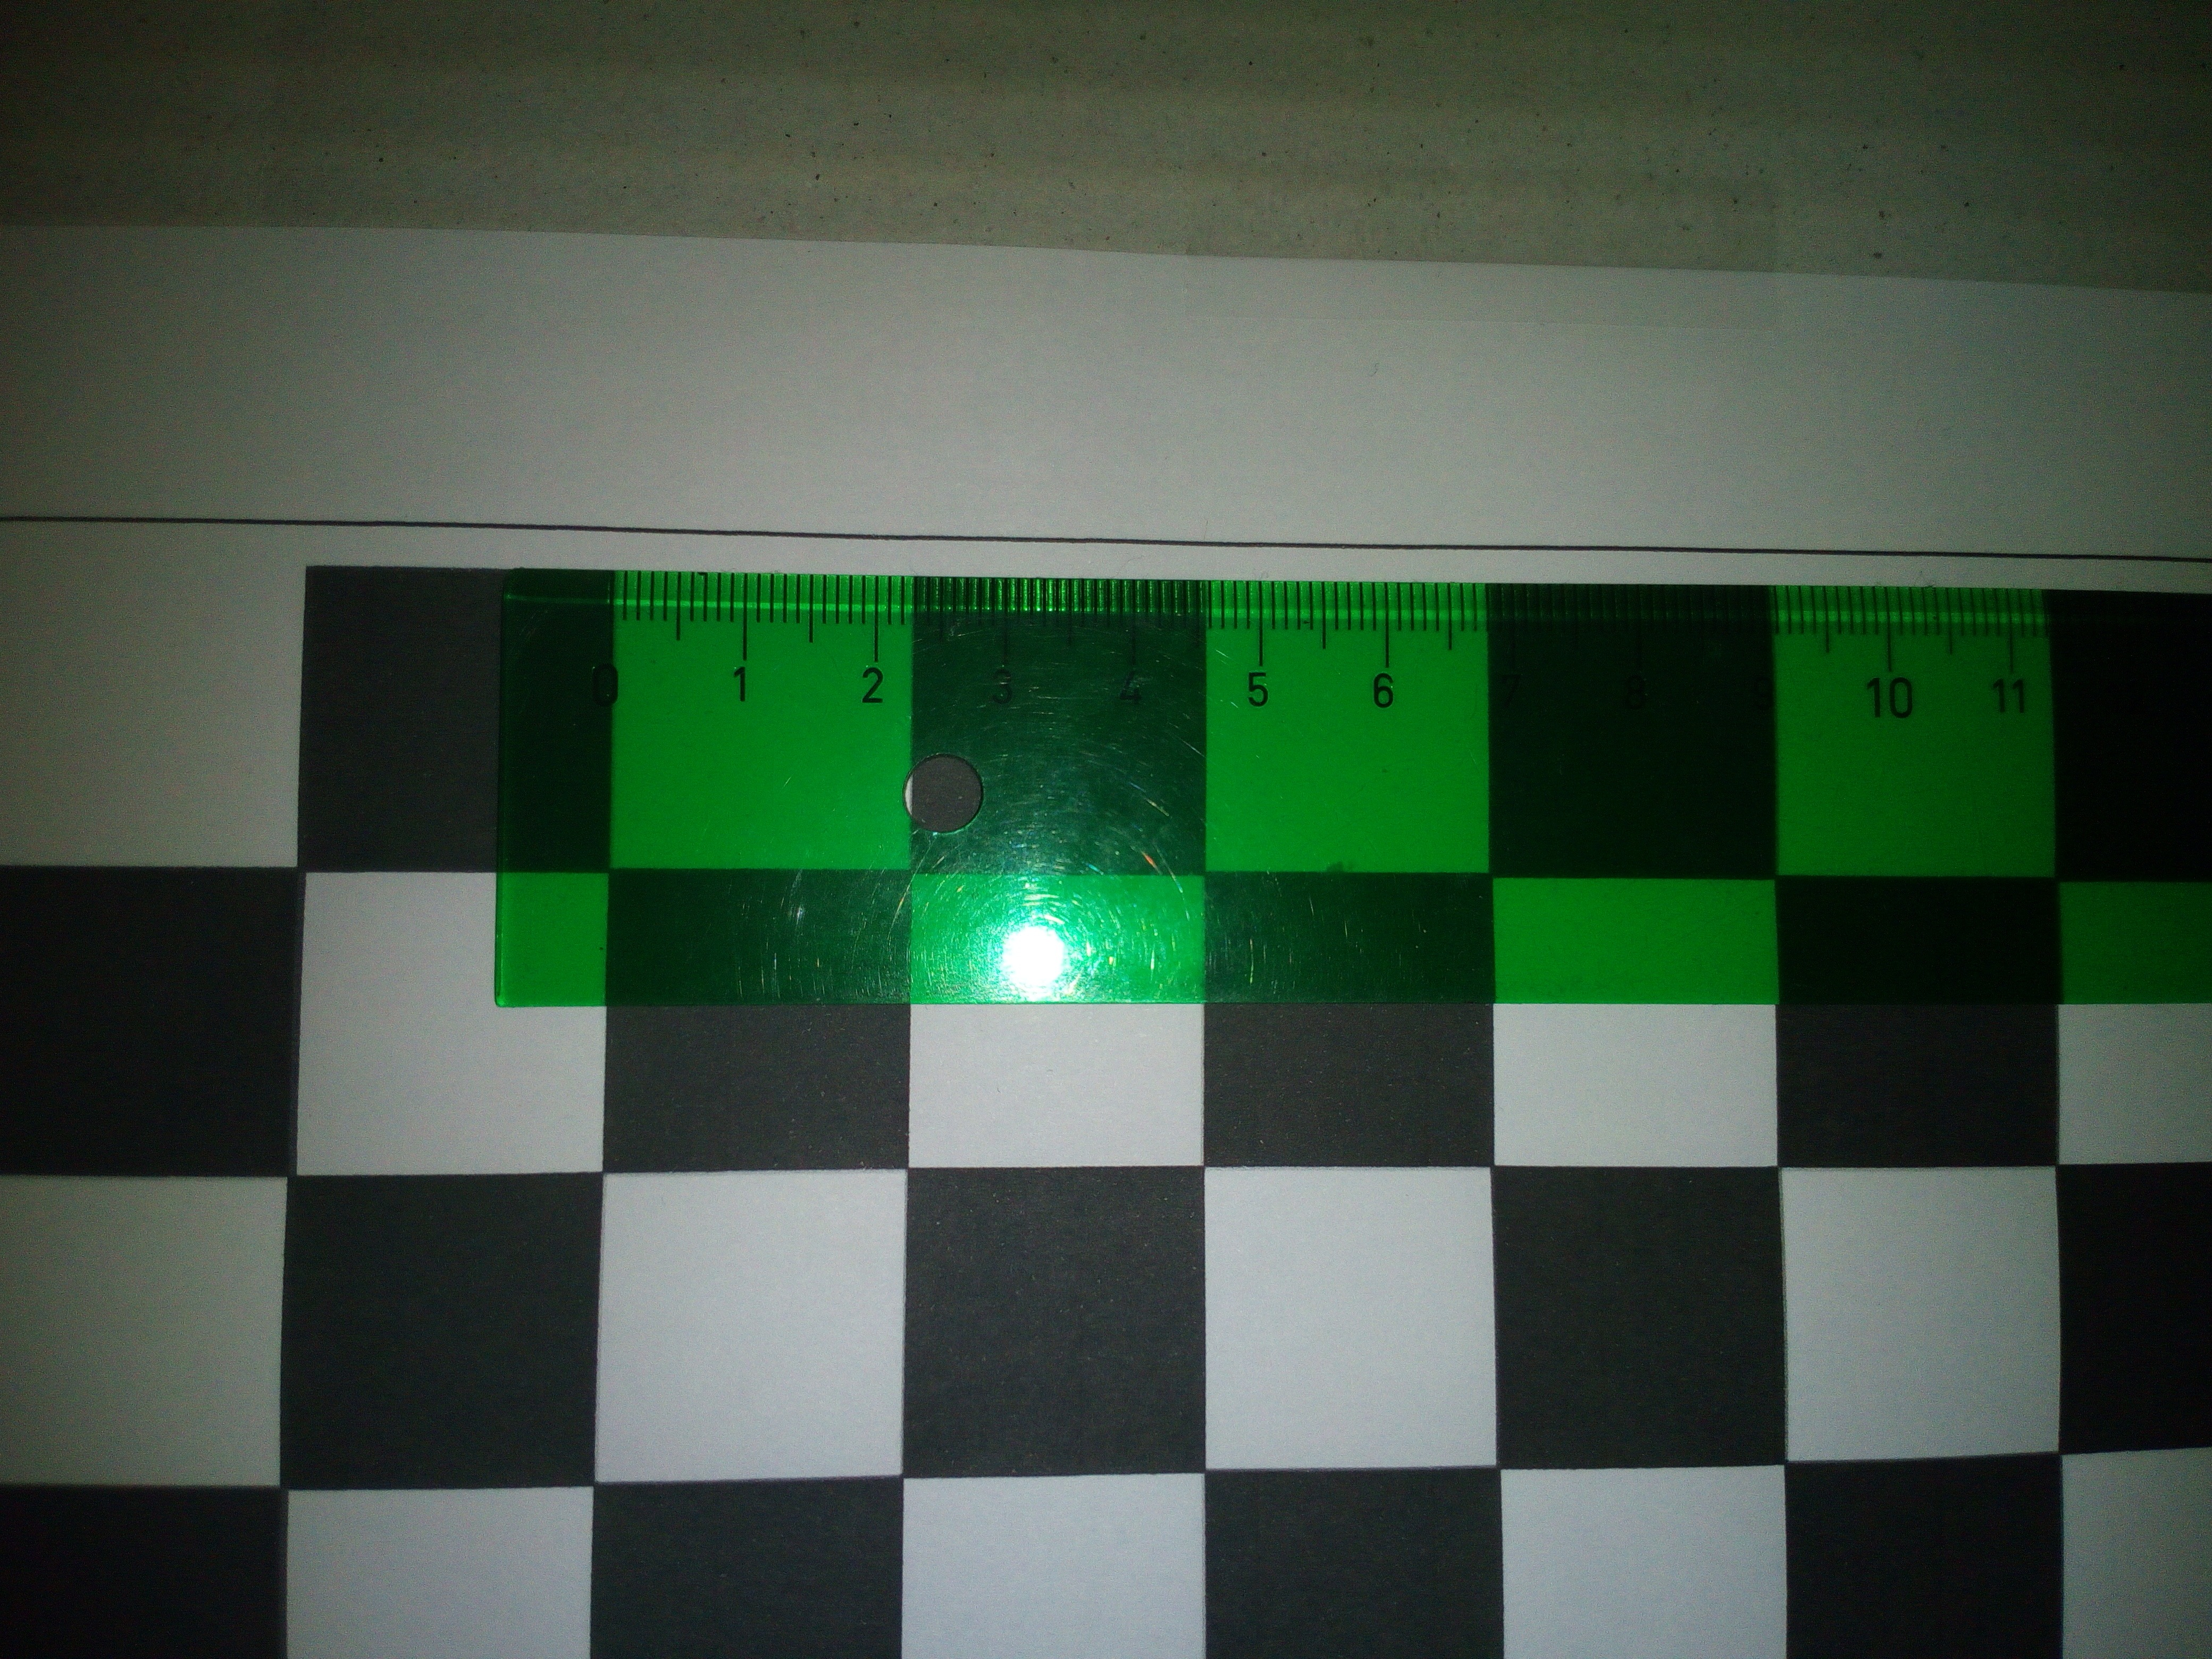
\includegraphics[scale = 0.05]{capitulo_03/figuras_dir/milimetros.jpg}
    \caption{Dimensión de los cuadrados de la plantilla}
    \label{fig: dimensioncuadrados}
    \end{figure}


    \item Función principal. Bucle de detección:

\begin{listing}[p]
\begin{minted}[bgcolor=bg,
               frame=lines,
               framesep=2mm,
               linenos]
               {C}
    Mat img, imgGray;
    bool found;

    for (int  i = 0; i < 14; i++){

	    imgs << direccion << i << ".jpg";
	    img = imread(imgs.str().c_str());
	    cvtColor(img, imgGray, COLOR_BGR2GRAY);
	    imgs=std::stringstream();

	    found = findChessboardCorners(imgGray,patternsize,corners2D, 
	                            CALIB_CB_ADAPTIVE_THRESH + 
	                            CALIB_CB_NORMALIZE_IMAGE + 
	                            CALIB_CB_FAST_CHECK);
	    if( found) {
	
		    cornerSubPix(imgGray, corners2D, Size(11, 11), Size(-1, -1), TermCriteria(TermCriteria::EPS + TermCriteria::COUNT, 30, 0.1 ));
		    drawChessboardCorners(img,patternsize,Mat(corners2D),found);
		    coord2D.push_back(corners2D);
		    coord3D.push_back(corners3D);
	    } 
	    namedWindow("image",WINDOW_AUTOSIZE);
	    imshow("image", img);
	    waitKey(1500);
    }

    cvDestroyWindow("image");
\end{minted}
\caption{Bucle de detección en ``calibration.cpp''}
\label{Lis: bucledeteccioncali}
\end{listing}
    
En cada iteración del bucle, se declara el nombre completo de cada imagen que posteriormente se lee con ``imread()’’ y se introduce en una matriz llamada ‘’img’’. Después, se llama a ``ctvColor()’’ que convierte la imagen leída en otra imagen en blanco y negro. Esta imagen se almacena en la matriz ``imgGray’’. Ésta última, se utiliza para encontrar el patrón con ``findChessboardCorners()’’ (``Listing \ref{Lis: bucledeteccioncali}''). Si encuentra un patrón en la plantilla, entonces dibuja las esquinas sobre la imagen y lo muestra con ``imshow()’’.  Si las imágenes no muestran este dibujo es debido a que no se ha detectado ningún patrón en la imagen y el proceso debe efectuarse de nuevo. Cuando se han mostrado todas las imágenes, se deja de mostrar la ventana de las capturas con ``cvDestroyWindow()’’.

    \item Función principal. Obtención de los parámetros de la cámara: 
    
\begin{listing}[p]
\begin{minted}[bgcolor=bg,
               frame=lines,
               framesep=2mm,
               linenos]
               {C} 
    Mat cameraMatrix = Mat::eye(3, 3, CV_64F);
    Mat distCoeffs = Mat::zeros(8, 1, CV_64F);
    std::vector<Mat> rvecs;
    std::vector<Mat> tvecs;
	
    double rms = calibrateCamera(coord3D, coord2D, img.size(), cameraMatrix,distCoeffs, rvecs, tvecs, 
				CALIB_FIX_PRINCIPAL_POINT + CALIB_FIX_ASPECT_RATIO + CALIB_ZERO_TANGENT_DIST,
				TermCriteria(CV_TERMCRIT_ITER + CV_TERMCRIT_EPS, 30, 2.22e-16));

    std::cout << "RMS: " << rms << std::endl;
    std::cout << "Camera matrix: " << cameraMatrix << std::endl;
    std::cout << "Distortion _coefficients: " << distCoeffs << std::endl;
\end{minted}
\caption{Obtención de los parámetros de la cámara}
\label{Lis: parametroscamara}
\end{listing}
    
Se declaran el número de precisión, la matriz de la cámara de orden 3, el vector de coeficientes de distorsión y los vectores de traslación y rotación (``Listing \ref{Lis: parametroscamara}''). ``calibrateCamera()’’ devuelve estos valores y los introduce en los objetos correspondientes. 
\clearpage
    \item Función principal. Guardado de los parámetros:
    
\begin{listing}[H]
\begin{minted}[bgcolor=bg,
               frame=lines,
               framesep=2mm,
               linenos]
               {C} 
    saveparams("//home//esther//Desktop//VKMS//Calibracion//MiCam.yml",cameraMatrix,distCoeffs,rvecs,tvecs,rms);
\end{minted}
\caption{Guardado de los parámetros}
\label{Lis: guardadoparametros}
\end{listing}
    
Los parámetros de la cámara se guardan llamando a ``saveparams()’’ especificando la ruta y el archivo ``.yml’’  donde se introducen.

\end{itemize}


%/////////////////// Subsubsección ///////////////////%
\subsubsection{Lectura del archivo de calibración MiCam.yml}\label{s3_2_2_3}

El archivo que almacena los parámetros de calibración tiene su utilidad. Cada vez que se desarrolle un programa que necesite la cámara para tomar medidas sobre las imágenes que captura no es necesario incluir el código de calibración, sino que basta con cargar este archivo y llamar a la función que utiliza los parámetros obtenidos en este proceso para corregir la distorsión radial.

Es por ello por lo que hay que realizar una ligera modificación en el código de Abner. Después de encender la cámara y comprobar si se ha detectado o no, el código se modifica como se muestra en ``Listing \ref{Lis: micamlectura}'': 

\begin{listing}[p]
\begin{minted}[bgcolor=bg,
               frame=lines,
               framesep=2mm,
               linenos]
               {C}
    cv::Mat frame;
    cv::Mat imageUndistorted;
    fifo = open("eye_fifo", O_WRONLY|O_CREAT, ~0);
    while (1)
    {
        cap >> frame; // outputs the webcam image to a Mat
        cv::Mat cameraMatrix = cv::Mat::eye(3, 3, CV_64F);
        cv::Mat Distortion = cv::Mat::zeros(8, 1, CV_64F);		
	    cv::FileStorage storageRead("MiCam.yml",    cv::FileStorage::READ);
	    storageRead["Camera_Matrix"] >> cameraMatrix;
	    storageRead["Distortion_Coefficients"] >> Distortion;
      
        undistort(frame, imageUndistorted, cameraMatrix, Distortion);//corrijo distorsion radial
      
  
        if (!imageUndistorted.data) break;
            detectEyes(imageUndistorted, faceCascade, eyeCascade);
            cv::imshow("Webcam", imageUndistorted); // displays the Mat
            if (cv::waitKey(30) >= 0) {
		        break;  // takes 30 frames per second. if the user presses any button, it stops from showing the webcam
		        close(fifo);
		    }
        }
  
        return 0;
    }
\end{minted}
\caption{Lectura del archivo ``MiCam.yml''}
\label{Lis: micamlectura}
\end{listing}
    
Después de abrir el archivo FIFO, comienza un bucle infinito que solo puede terminar cuando se presiona alguna tecla. En cada iteración, se introduce la imagen capturada en una matriz llamada ``frame’’. Después, se procede a la lectura del archivo que contiene los parámetros (``MiCam.yml’’) con `` storageRead()’’ y a continuación, se usa esta misma función para encontrar en el archivo la matriz de la cámara y los coeficientes de distorsión y rellenar las correspondientes matrices con los datos recogidos del archivo. Una vez hecho esto, se invoca a ``undistort()’’. Su finalidad consiste en tomar la matriz de la cámara y los coeficientes de distorsión y a partir de la imagen original (matriz ``frame’’) realizar la corrección eliminando la distorsión e introduciendo la imagen corregida en otra matriz denominada `` imageUndistorted’’. En base a la imagen corregida se realizan el resto de operaciones de detección como se relata en la sección 3.2.3.
\clearpage

%%%%%%%%%%%%%%%%%%%%%%%%%%%%%%%%%%%%%%%%%%%%%%%%%%%%%%%
%		            	Seccion          			  %
%%%%%%%%%%%%%%%%%%%%%%%%%%%%%%%%%%%%%%%%%%%%%%%%%%%%%%%
\section{Programa de selección} \label{s3_4}

%%%%%%%%%%%%%%%%%%%%% Subsección %%%%%%%%%%%%%%%%%%%%%
\subsection{Descripción de ``selector.c''} \label{s3_4_1}

El programa de selección se divide esencialmente en tres partes: Obtención de eventos del archivo FIFO en el que fueron almacenados en ``eye\_detect.cpp'', comprobación de la región en la que se encuentra la coordenada {\itshape x} del ojo y escritura del resultado en otro archivo FIFO que será posteriormente leído por el programa cliente de la conexión TCP. La forma en la que se leen los eventos del archivo FIFO es igual que la forma en la que se leen del archivo de interfaz USB HID (``Hidraw''), es decir, se declara un manejador de tipo ``event\_handlder()''  que retorna una función que crea el manejador y toma como argumentos el descriptor del archivo y la función ``eye()''. Cada vez que el bucle de eventos ceda el control al manejador, ``eye()'' se encarga de leer el descriptor las veces necesarias hasta que ``contador'' valga 5 (bucle ``while''). En cada una de esas lecturas, se verifica si la lectura se ha realizado con éxito (para ello, ``s'' debe ser positiva) y comprueba si ese evento leído es del ojo. Esto quiere decir que si el evento corresponde al centro del iris (cuyo evento va precedido del carácter ``P''), no se toma en cuenta. En caso de que sea un evento del ojo, el puntero a un objeto de tipo ``eyetracking'' definido con el nombre ``e'' se iguala al búfer o vector en el que se han introducido los datos leídos. En este caso, es necesario introducir un cast para forzar la igualdad de ambos. De esta forma, ``e'' ahora apunta al bufer que ha sido convertido a un objeto cuyos atributos son el tipo de evento, las coordenadas {\itshape x} e {\itshape y} del punto de la esquina superior izquierda del recuadro que encuadra el área del ojo izquierdo de la imagen y el lado de dicho recuadro, d. Es importante destacar que las coordenadas del recuadro que encierra el ojo derecho no se necesitan porque solamente se consideran los cambios que se producen en la coordenada x del punto superior izquierdo del recuadro del ojo izquierdo de la imagen. La coordenada {\itshape x} del recuadro del ojo derecho no suele tomar un valor inferior a 70\footnote{Véase la sección 4.5}, por eso, todos aquellos valores de {\itshape x} que son inferiores a 70 se almacenan en un vector de 5 posiciones. Cada vez que se introduzca un valor en este vector, el contador se incrementa hasta valer 5, momento en el cual el bucle termina y se realiza la suma de todos estos valores, dividiéndose posteriormente por 5 para hallar la media de los mismos y así obtener un resultado estable ignorando en la medida de lo posible las posibles desviaciones en las muestras. Posteriormente, se llama a la función ``function()'' que, en primer lugar, comprueba la posición de la pantalla (derecha o izquierda) determinado en la variable ``pantalla'' con un carácter. Después, en función de cada caso, analiza en qué conjunto de valores se encuentra la media de la coordenada x hallada anteriormente comparándola con los valores de las variables ``x1'' y ``x2'' que se han obtenido experimentalmente\footnote{Véase la sección 4.5}. Cuando se detecta que el usuario se mantiene mirando al frente, independientemente de donde se encuentra la pantalla secundaria, la función retorna ``A''. En cambio, cuando se detecta que el usuario gira la cabeza a uno de los dos lados, la función devuelve ``B''. Estos caracteres se almacenan en la variable ``salida'' que se introduce en un archivo FIFO de nombre ``select'' con la función de escritura {\itshape write()}. Si no es posible introducir estos valores, el bucle de eventos finaliza llamando a ``reactor\_quit()''.

\begin{listing}[H]
\begin{minted}[bgcolor=bg,
               frame=lines,
               framesep=2mm,
               linenos]
               {C}

    #include <reactor/reactor.h>
    #include <reactor/console.h>
    #include <stdio.h>
    #include <unistd.h>
    #include <assert.h>
    #include <sys/types.h>
    #include <sys/stat.h>
    #include <fcntl.h>
    #include <sys/select.h>
    
    ////////////// Media de la distancia X de O' a 0'' //////////////
    
    // 		Mirada central: 45,46,47,48,49,50,51
    // 		Mirada derecha: 59,60,61,62,63
    // 		Mirada izquierda: 40,41,42,43,44
    
    #define x1 44
    #define x2 59
    
    typedef struct {
    	char tipo;
    	int x, y, d;
    } eyetracking;
    
    eyetracking* e;
\end{minted}
\caption{Continuación de ``Listing \ref{Lis: programaselector}''}
%\label{Lis: programaselector}
\end{listing}

\clearpage
\begin{listing}[H]
\begin{minted}[bgcolor=bg,
               frame=lines,
               framesep=2mm,
               linenos]
               {C}
    
	static void eye (event_handler* ev);

	event_handler* eye_handler_new(int fifo) {
		return event_handler_new(fifo, eye);
	}
	
	char function (double media) {
	char salida;
	char pantalla= 'I'; // Posicion de la pantalla secundaria
	
	switch (pantalla) {
		case 'D':
			if (media>=x2) {
				salida= 'B';
			} 
			else {
				salida = 'A';
			}
			break;
			break;
		case 'I': 
			if (media<=x1) {
				salida = 'B';
			}
			else {
				salida= 'A';
			}	
			break;
			break;
	}

	return salida;
}

\end{minted}
\caption{Continuación de ``Listing \ref{Lis: programaselector}''}
%\label{Lis: programaselector}
\end{listing}

\begin{listing}[p]
\begin{minted}[bgcolor=bg,
               frame=lines,
               framesep=2mm,
               linenos]
               {C}
	static void eye (event_handler* ev) {
		
		int contador=0;
		int vector[5];
		int valor =0;
		
		while (contador<5) { 
		int s;
		char buf[512];
		s= read (ev->fd, buf, sizeof(buf));
		printf("s: %d\n", s);
		
			if (s <0)
			reactor_quit(ev->r);
		
			
			if (buf[0] == 'E') {
				e = (eyetracking*)buf;

				if (e->x < 70) {
				vector[contador]= e->x;
				contador++;
				}
			}
		}
	for (int i=0; i<contador+1; i++) {
		
		valor= valor + vector[i];
		
	}

	double MM= (double) valor/5;
	char salida = function(MM);
\end{minted}
\caption{Continuación de ``Listing \ref{Lis: programaselector}''}
%\label{Lis: programaselector}
\end{listing}
	

\begin{listing}[p]
\begin{minted}[bgcolor=bg,
               frame=lines,
               framesep=2mm,
               linenos]
               {C}
	int fifo2= -1;	
	fifo2 = open("select", O_RDWR);

	int p;
	char buf1[1];
	buf1[0]= salida;
	p= write (fifo2, buf1, sizeof(buf1));
	
		if (p <0)
		reactor_quit(ev->r);
		
	printf("Salida introducida: %c\n", salida);
    close(fifo2);
	}
	
	int main () {
		

		int fifo1= -1;
		fifo1 = open("/home/esther/Desktop/VKMS/Recopilacion/Eye_tracking/eye_fifo", O_RDONLY);
		printf("fifo1: %d\n",fifo1);
		
		void* state= console_set_raw_mode(0);
		reactor *r= reactor_new();
		reactor_add(r, eye_handler_new(fifo1));
		reactor_run(r);
		console_restore(0,  state);
		close(fifo1);
		return 0;
	}
\end{minted}
\caption{Programa ``Selector.c''}
\label{Lis: programaselector}
\end{listing}


%%%%%%%%%%%%%%%%%%%%% Subsección %%%%%%%%%%%%%%%%%%%%%
\subsection{Obtención de las coordenadas {\itshape x} límite} \label{s3_4_2}

Existen varias formas de determinar la dirección de la mirada del usuario. Una de las más sencillas consiste en analizar el cambio que se produce en las coordenadas del punto O'' (correspondiente al recuadro del ojo izquierdo) respecto a O' (correspondiente al recuadro de la cara). Cuando el usuario mira al frente, la distancia medida en el eje X de O' respecto O'' tiene cierto valor. Dicho valor cambia cuando la persona gira la cabeza hacia un lado u otro. Este gesto es el más común en aquellos que quieran centrar la atención en otro monitor distinto al principal. Es lógico que en este análisis solo se estudie los cambios de {\itshape x} puesto que los cambios en {\itshape y} son insignificantes debido a que la rotación de la cabeza se produce en torno a un eje vertical.

Para estudiar esta situación, se ejecuta el programa ``eye\_detect.cpp''\footnote{Véase la sección 4.3.}. Como ya se ha comentado, muestra las capturas detectadas con la cámara de Raspberry Pi, y sobre ellas, dibuja las regiones detectadas por el algoritmo de Viola-Jones. Observar la posición de los recuadros es fundamental para determinar la variación que se produce en la coordenada {\itshape x}. Todo este proceso se relata en la sección 4.5 junto a los resultados.


%%%%%%%%%%%%%%%%%%%%%%%%%%%%%%%%%%%%%%%%%%%%%%%%%%%%%%%
%		            	Seccion          			  %
%%%%%%%%%%%%%%%%%%%%%%%%%%%%%%%%%%%%%%%%%%%%%%%%%%%%%%%
\section{Comunicaciones Raspberry Pi - Arduino} \label{s3_5}

Tras introducir el carácter que indica el equipo que recibe los eventos y obtener los eventos de los dispositivos de control, el siguiente paso consiste en establecer una comunicación entre el microcontrolador central con cada Arduino Leonardo. Para ello, el libro del taller dispone de un programa cliente y otro programa servidor, ambos TCP y UCP. Debido a lo expuesto en la sección 2.3 de conceptos teóricos, se prefiere una conexión TCP para asegurar la recepción de los datos sin errores, lo cual otorga mayor estabilidad al sistema de comunicación. Por ello, se toma el programa cliente TCP para modificarlo en función de la aplicación. Asimismo, para que Arduino tenga el rol de servidor, tiene que implementarse un programa o también llamado ``sketch'' en el entorno de desarrollo Arduino. Hay que tener claro el tipo de módulo que se emplea para conectarse a la red. Se diferencian principalmente en dos tipos: módulos Ethernet y módulos Wifi. En este caso, se implementa con un módulo Ethernet genérico o ``Ethernet Shield''.


%%%%%%%%%%%%%%%%%%%%% Subsección %%%%%%%%%%%%%%%%%%%%%
\subsection{Raspberry Pi como cliente: ``Cliente.c''} \label{s3_5_1}

%/////////////////// Subsubsección ///////////////////%
\subsubsection{Apertura del descriptor de eventos del teclado y del ratón}\label{s3_5_1_1}

El programa cliente del taller toma aquello introducido en el teclado mediante ``fgets()'' leyendo el descriptor de la entrada estándar\footnote{Véase el anexo B.}. En este caso, no interesa en absoluto el descriptor del teclado, lo único que interesa es abrir el archivo especial ``archivo'' y tomar el descriptor resultante que se emplea para obtener aquellos eventos HID introducidos por ``mk.c'' mediante la operación de escritura. El procedimiento para adquirir el contenido del archivo FIFO es igual al que se emplea los archivos descriptores de la interfaz USB HID: en primer lugar, se abre el archivo para conseguir el descriptor con {\itshape open()} y en segundo lugar, se emplea el descriptor para leer el contenido con {\itshape read()}. 

\begin{listing}[H]
\begin{minted}[bgcolor=bg,
               frame=lines,
               framesep=2mm,
               linenos]
               {C}

///////////////////////////////////////////////////////////////
//	OBTENCIÓN DE EVENTOS DE TECLADO Y RATON		        //
///////////////////////////////////////////////////////////////
	
int fifo1= -1;
unsigned char bufer2[1025];
fifo1= open("/home/esther/Desktop/VKMS/Recopilacion/Eventos_mk/archivo", O_RDONLY);
int s;
s= read (fifo1, bufer2, sizeof(bufer2));
printf("numero de bytes leidos: %d\n", s);

\end{minted}
\caption{Obtención de los eventos del teclado y ratón a partir del descriptor de archivo.}
\label{lst:hid-events-read-fd}
\end{listing}

Tras realizar estas dos llamadas al sistema, el vector ``bufer2'' contiene los bytes que constituyen el evento que ha entrado primero al archivo FIFO y que, por lo tanto, es el primero en leerse. El número de bytes almacenados en ``bufer2'' es igual al número de bytes leídos independientemente del tamaño  de 1025 bytes asignado al vector. El hecho de declarar el vector con el tipo ``unsigned char'' permite que cada byte pueda ser obtenido en decimal como un valor positivo desde 0 hasta 255, lo que se diferencia de un simple ``char'' ya que al representar en el terminal una variable de este tipo en hexadecimal, se puede obtener el número precedido de ``ffffff'' indicando que el número es negativo. Sin embargo, ambas opciones son válidas.

%/////////////////// Subsubsección ///////////////////%
\subsubsection{Selección del Arduino de destino}\label{s3_5_1_2}

Otra de las funciones de este programa es tomar el carácter enviado por el programa ``selector.c'' (``Listing \ref{lst:hid-event-demux}''). Esta decisión es concluyente a la hora de dictaminar la dirección IP de destino. El procedimiento es igual al anterior, se abre el archivo FIFO ``select'' y se lee posteriormente. El carácter ocupa un byte que se almacena en la única posición del vector ``bufer3''. A continuación, mediante una claúsula ``if'' se evalúa el contenido del vector asignando el valor de uno de los dos descriptores de la conexión a la variable ``descriptor'' que se emplea posteriormente para enviar información mediante {\itshape write()}.

\begin{listing}[p]
\begin{minted}[bgcolor=bg,
               frame=lines,
               framesep=2mm,
               linenos]
               {C}
///////////////////////////////////////////////////////////////
//   OBTENCION DEL ARDUINO AL QUE HAY QUE ENVIAR EVENTOS     //
///////////////////////////////////////////////////////////////
	
	
int fifo2= -1;
int descriptor;
char bufer3[1];
fifo2= open("/home/esther/Desktop/VKMS/Recopilacion/Selector/select", O_RDONLY);
int r;
r= read (fifo2, bufer3, sizeof(bufer3));
	
if (bufer3[0]=='A') {
		
	descriptor= fd1;
		
} else if (bufer3[0]=='B') {
		
	descriptor=fd2;
} 

\end{minted}
\caption{Selección del Arduino que recibe los eventos HID.}
\label{lst:hid-event-demux}
\end{listing}

%/////////////////// Subsubsección ///////////////////%
\subsubsection{Escritura en el descriptor del servidor}\label{s3_5_1_3}

La función {\itshape write()} usa el descriptor de la conexión para enviar el contenido de ``bufer2''. El número de bytes que envía corresponden con el número de bytes que se leen referentes a los eventos (variable ``s''). 

\begin{listing}[H]
\begin{minted}[bgcolor=bg,
               frame=lines,
               framesep=2mm,
               linenos]
               {C}

////////////////////////////////////////////////////////////////////////////
//   ENVIO DE LOS EVENTOS DE TECLADO Y RATON AL ARDUINO CORRESPONDIENTE   //
////////////////////////////////////////////////////////////////////////////
	
int n = write(descriptor, bufer2, s); //strlen(bufer2)
assert(n >= 0);
if (n == 0) {
	break;
	close(fifo1);
	close(fifo2);
}

\end{minted}
\caption{Envío de los eventos HID.}
\label{lst:hid-event-send}
\end{listing}

En cuanto a los descriptores de la conexión ``fd1'' y ``fd2'', se adquieren a partir de la llamada a la función ``tcp\_client\_socket()'' que contiene como argumentos la dirección IP del servidor Arduino y el puerto de conexión.


\begin{listing}
\begin{minted}[bgcolor=bg,
               frame=lines,
               framesep=2mm,
               linenos]
               {C}

const char* IP1;
	IP1= "192.168.1.45";
const char* IP2;
	IP2= "192.168.1.46";
	
	int fd1 = tcp_client_socket(IP1, "1000"); 
	int fd2 = tcp_client_socket(IP2, "1000");

\end{minted}
\caption{Adquisición de los descriptores de la conexión.}
\label{lst:client-socket-create}
\end{listing}


%%%%%%%%%%%%%%%%%%%%% Subsección %%%%%%%%%%%%%%%%%%%%%
\subsection{Arduino como servidor: ``Servidor\_TCP.ino''} \label{s3_5_2}

Este ``sketch'' se divide en tres partes según su función: conexión, lectura de los eventos recibidos y simulación de pulsaciones y movimientos del ratón a partir de los mismos. En esta sección se analizan las dos primeras partes debido a que la última se considera objeto de estudio por separado\footnote{Véase la sección 3.5.}.

%/////////////////// Subsubsección ///////////////////%
\subsubsection{Conexión y establecimiento del servidor}\label{s3_5_2_1}

Tal y como se ha indicado, se usa un módulo Ethernet y es por eso por lo que es necesario incluir la biblioteca Ethernet a través del archivo cabecera ``Ethernet.h''. Ya que Arduino se debe conectar de alguna manera al módulo, se incluye otro archivo más, ``SPI.h'', necesario para establecer una conexión via SPI entre ambos circuitos integrados. Posteriormente, se define la cadena de bytes ``mac'' y la dirección IP del servidor. Mediante la clase ``EthernetServer'' se declara como servidor la variable ``ArduinoTCP'' y a continuación, dentro de ``setup()'' se inicializan todos aquellos parámetros una sola vez: se establece la tasa de baudios o ``baud rate'' del puerto serie y se inicia la comunicación con ``Ethernet.begin()'' y el servidor TCP (``Listing \ref{lst:arduino-ethernet}'').

\begin{listing}
\begin{minted}[bgcolor=bg,
               frame=lines,
               framesep=2mm,
               linenos]
               {C}

#include <SPI.h>
#include <Ethernet.h>
//#include <Keyboard.h>
//#include <Mouse.h>

byte MiMac[]= {0xDE, 0xAD, 0xBE, 0xEF, 0xFE, 0xED};

byte MiIp[]= {192,168,1,45};

EthernetServer ArduinoTCP = EthernetServer (1000);

void setup() {

Serial.begin(9600);
Serial.println("Initializing ethernet connection");
Ethernet.begin(MiMac, MiIp);
ArduinoTCP.begin();
// Keyboard.begin();  
}

\end{minted}
\caption{Conexión de Arduino a Internet mediante un módulo Ethernet.}
\label{lst:arduino-ethernet}
\end{listing}


%/////////////////// Subsubsección ///////////////////%
\subsubsection{Lectura de los eventos}\label{s3_5_2_2}

Invocando a ``cliente.read()'' se obtiene uno de los bytes de los eventos enviados por el cliente de la conexión. Estos constituyen en total 7 bytes para el ratón y 1 byte para el teclado aunque depende del hardware y/o sistema operativo que se usa. Al igual que los eventos oculares, cada uno de ellos va precedido por un carácter para distinguir si se tratan de datos obtenidos por el ratón o por el teclado, de ahí que la estructura del evento sea ``TX'' y ``RXXXXXXX'' siendo ``X'' la representación de un byte. Para realizar un sistema de lectura de eventos, se ha pensado en un vector de 8 posiciones de tipo ``byte'', en el que, en cada iteración de un bucle infinito, los valores de cada posición se recorran hacia la posición sucesora y sea la posición ``0'' la que renueva su valor en cada iteración mediante una llamada a ``cliente.read()'' para recibir un nuevo byte. A su vez, en cada iteración, se evalúa la última posición del vector. Esto quiere decir que comprueba si el byte corresponde al carácter ``T'' o ``R''. En el primer caso, lee la posición anterior a la última, ya que siempre se envía primero el carácter del tipo de evento seguido del carácter referente a la tecla pulsada. En el segundo caso, comienza un bucle de 7 iteraciones de tipo regresivo en el que se comparan todos los valores de cada una de las posiciones desde aquella anterior a la última hasta la primera con aquellas cadenas definidas como los atributos de un objeto llamado ``raton'' de tipo ``eventos''. Dado que estas cadenas están inicializadas en un orden opuesto al de verificación, las posiciones no pueden ser regresivas. Esto quiere decir que el valor relativo a la posición 6 del bufer de evento, ``buf'', no se puede comparar con el valor de la posición 6 de cualquiera de los vectores que componen el objeto ``ratón''. Así pues, ``buf[6]'' se le compara con la posición 0 de otro vector, ``buf[5] se compara con la posición 1 de otro vector y así sucesivamente. Para ello, se inicializa a 0 una variable llamada ``p'' que incrementa su valor la unidad en el momento en el que finaliza una iteración del bucle.

Cada atributo es un vector que contiene los bytes de los eventos más significativos con los que posteriormente se va a realiza la simulación:

\begin{itemize}
    \item {\bfseries Movimiento en sentido positivo a través del eje X}: ``{0x3, 0x0, 0x1, 0x0, 0x0, 0x0, 0x0}''.
    \item {\bfseries Movimiento en sentido negativo a través del eje X}: ``{0x3, 0x0, 0xFF, 0xF, 0x0, 0x0, 0x0}''.
    \item {\bfseries Movimiento en sentido positivo a través del eje Y}: ``{0x3, 0x0, 0x0, 0xF0, 0xFF, 0x0, 0x0}''.
    \item {\bfseries Movimiento en sentido negativo a través del eje Y}: ``{0x3, 0x0, 0x0, 0x10, 0x0, 0x0, 0x0}''.
    \item {\bfseries Cliqueo sobre el botón derecho del ratón}: ``{0x3, 0x2, 0x0, 0x0, 0x0, 0x0, 0x0}''.
    \item {\bfseries Cliqueo sobre el botón izquierdo del ratón}: ``{0x3, 0x1, 0x0, 0x0, 0x0, 0x0, 0x0}''.
\end{itemize}

Estos valores se obtienen de la experiencia.
Cada vez que coincide un valor de ``buf'' con uno de cualquiera de los vectores, se incrementa el valor del contador correspondiente.
Cuando todos los valores de ``buf'' coinciden con los de uno de estos vectores, el contador vale 7 y es mayor que cualquier otro de los contadores. Cuando esto sucede, Se da un valor a ``A'' y ``B'' que constituyen los argumentos de ``mouse.move()''\footnote{Véase la sección 3.5.}. Cuando finaliza el bucle, todas las variables se inicializan a cero y comienza de nuevo el proceso. 

A continuación se representa el programa ``Servidor\_TCP.ino'' en ``Listing \ref{lst:servidor-tcp-ino}''. Cabe destacar que todos los comentarios de código hacen referencia a funciones de simulación de las que se habla en la siguiente sección.



\begin{listing}[p]
\begin{minted}[bgcolor=bg,
               frame=lines,
               framesep=2mm,
               linenos]
               {C}

#include <SPI.h>
#include <Ethernet.h>
//#include <Keyboard.h>
//#include <Mouse.h>

byte MiMac[]= {0xDE, 0xAD, 0xBE, 0xEF, 0xFE, 0xED};

byte MiIp[]= {192,168,1,45};

EthernetServer ArduinoTCP = EthernetServer (1000);

void setup() {

Serial.begin(9600);
//pinMode(10,OUTUPUT)
Serial.println("Initializing ethernet connection");
Ethernet.begin(MiMac, MiIp);
ArduinoTCP.begin();
// Keyboard.begin();  
}


unsigned char buf[8]={0x0,0x0,0x0,0x0,0x0,0x0,0x0,0x0};

#define sensitivity 200

typedef struct eventos {  
    byte x_plus[7]= {0x3, 0x0, 0x1, 0x0, 0x0, 0x0, 0x0};
    byte x_less[7]= {0x3, 0x0, 0xFF, 0xF, 0x0, 0x0, 0x0};
    byte y_plus[13]= {0x3, 0x0, 0x0, 0xF0, 0xFF, 0x0, 0x0};
    byte y_less[7]= {0x3, 0x0, 0x0, 0x10, 0x0, 0x0, 0x0};
    byte ckd[7]= {0x3, 0x2, 0x0, 0x0, 0x0, 0x0, 0x0};
    byte cki[7]= {0x3, 0x1, 0x0, 0x0, 0x0, 0x0, 0x0};
};

\end{minted}
\caption{Continuación de ``Listing \ref{lst:servidor-tcp-ino}''}
%\label{lst:servidor-tcp-ino}
\end{listing}


\begin{listing}[p]
\begin{minted}[bgcolor=bg,
               frame=lines,
               framesep=2mm,
               linenos]
               {C}
void loop() {
    eventos raton;
    EthernetClient cliente = ArduinoTCP.available();
    
    //char c;
    int i,p;
    int cont1=0;
    int cont2=0;
    int cont3=0;
    int cont4=0;
    int cont5=0;
    int cont6=0;
    double A=0;
    double B=0;
      

    Serial.print("Contenido de buf[0]: ");
    Serial.println(buf[0], HEX); 
    
    buf[0]= cliente.read(); 
    
    //////////////////////////////////////////////
    //        Leer el contenido del bufer       //
    //////////////////////////////////////////////
    
    if (buf[7]=='T') {
        //Keyboard.write(buf[6]);
        Serial.print("Caracter: ");
        Serial.println(buf[6], HEX);
    }

    if  (buf[7]=='R') {
        for (i=6; i>=0; i--) {
            if (buf[i]==raton.x_plus[p]) {
                cont1++;
                if (cont1==7) {
                    A= (510/sensitivity);
                    B=0;
                    Serial.println("A");
                }
            }
\end{minted}
\caption{Continuación de ``Listing \ref{lst:servidor-tcp-ino}''}
%\label{lst:servidor-tcp-ino}
\end{listing}
            
\begin{listing}[p]
\begin{minted}[bgcolor=bg,
               frame=lines,
               framesep=2mm,
               linenos]
               {C}         
            if (buf[i]==raton.x_less[p]) {
                cont2++;;
                if (cont2==7) {
                    A= (510/sensitivity)*(-1);
                    B=0;
                    Serial.println("B");
                }
            }
            if (buf[i]==raton.y_plus[p]) {
                cont3++;
                if (cont3==7) {
                    A= 0;
                    B= (510/sensitivity);
                    Serial.println("C");
                }
            }
            if (buf[i]==raton.y_less[p]) {
                cont4++;
                if (cont4==7) {
                    A= 0;
                    B= (510/sensitivity)*(-1);
                    Serial.println("D");
                }
            }
            if (buf[i]==raton.ckd[p]) {
                cont5++;
                if (cont5==7) {
                    //Mouse.press(MOUSE_RIGHT);  
                    //delay(200);
                    //Mouse.release(MOUSE_RIGHT);
                    Serial.println("E");
                }
            }

\end{minted}
\caption{Continuación de ``Listing \ref{lst:servidor-tcp-ino}''}
%\label{lst:servidor-tcp-ino}
\end{listing}
    
\begin{listing}[p]
\begin{minted}[bgcolor=bg,
               frame=lines,
               framesep=2mm,
               linenos]
               {C}   
                if (buf[i]==raton.cki[p]) {
                cont6++;
                if (cont6==7) {
                    //Mouse.press(MOUSE_LEFT);  
                    //delay(200);
                    //Mouse.release(MOUSE_LEFT);
                    Serial.println("F");
                }
            }
            p++;
       }
       //mouse.move(A,B,0);
    }
    //////////////////////////////////////////////
    //              Rellenar el bufer           //
    //////////////////////////////////////////////
    
    for (int i=7; i>0; i--) {
      //Serial.println("///////////////");
      Serial.print("Contenido de la posición ");  
      Serial.print(i); 
      Serial.print(" de buf[]: "); 
      Serial.println(buf[i], HEX);    
      buf[i]= buf[(i-1)];      
      delay(10);
    }
    Serial.println("///////////////");
      //Serial.println("buf[0]");
      //Serial.println(buf[0]);  
      //buf[0]= cliente.read();
      
    delay (2000);
}
\end{minted}
\caption{Programa ``Servidor\_TCP.ino''}
\label{lst:servidor-tcp-ino}
\end{listing}
\clearpage

%%%%%%%%%%%%%%%%%%%%%%%%%%%%%%%%%%%%%%%%%%%%%%%%%%%%%%%
%		            	Seccion          			  %
%%%%%%%%%%%%%%%%%%%%%%%%%%%%%%%%%%%%%%%%%%%%%%%%%%%%%%%
\section{Simulación de teclas en Arduino} \label{s3_6}

Los eventos recibidos se deben traducir como pulsaciones y movimientos de ratón reales. Esto se consigue simulándolo. Para ello, existen dos funciones principales: ``keyboard.write()'' y ``mouse.move()''.

%%%%%%%%%%%%%%%%%%%%% Subsección %%%%%%%%%%%%%%%%%%%%%
\subsection{Teclado} \label{s3_6_1}

Para simular las teclas pulsadas se emplea ``keyboard.write()''. Sin embargo, en primer lugar, es necesario que el programa cargue la biblioteca Keyboard mediante ``keyboard.h''. En segundo lugar, como Arduino es detectado como un dispositivo USB HID, el equipo debe identificarlo como un teclado. Por eso, se inicia una sola vez esta función a través de la llamada a ``keyboard.begin()''. Tras esto, es fácil simular las pulsaciones con ``keyboard.write()'' cuya función tiene como argumento el carácter que se recoge en ``buf'' mediante ``cliente.read()'' en el programa ``Servidor\_TCP.ino''.

%%%%%%%%%%%%%%%%%%%%% Subsección %%%%%%%%%%%%%%%%%%%%%
\subsection{Ratón} \label{s3_6_2}

Al igual que con el teclado, para simular los movimientos y ``clicks'' del ratón también hay que cargar la biblioteca correspondiente con ``mouse.h''. Para simular los movimientos en dos direcciones se emplea ``mouse.move()''. Sus argumentos hacen referencia al desplazamiento en el eje X y en el eje Y y al movimiento de la ruleta central respectivamente. Además de los datos relativos a desplazamientos, se pueden simular las pulsaciones de los botones laterales mediante ``mouse.press()'' para simular un botón presionado y ``mouse.release()'' para dejar de simular la pulsación, es decir, la primera función representa el cambio de estado de alto a bajo y la segunda, el cambio de bajo a alto de nuevo (estado inicial).















